\documentclass[portuguese,oneside]{tcc}

\usepackage{graphicx}
\usepackage{multirow}
\usepackage{nicefrac}
\usepackage{calc}
\usepackage{enumitem}
\usepackage{algpseudocode}
\usepackage{listings}
\usepackage{lipsum}
\usepackage{pdfpages}
\usepackage{minted}
\usepackage{xargs}
\usepackage{xcolor}
\usepackage[colorinlistoftodos,prependcaption,textsize=normalsize]{todonotes}
\usepackage{dirtree}
\usepackage{float}

\usemintedstyle{colorful}

\newfloat{listing}{thp}{lop}
\floatname{listing}{Listagem}

\newcommand{\green}[0]{\cellcolor[HTML]{67FD9A}}
\newcommand{\argmin}[1]{\underset{#1}{\operatorname{arg}\,\operatorname{min}}\;}
\newcommand{\argmax}[1]{\underset{#1}{\operatorname{arg}\,\operatorname{max}}\;}

\newcommandx{\unsure}[2][1=]{\todo[linecolor=red,backgroundcolor=red!25,bordercolor=red,#1,inline]{#2}}

\lstset{basicstyle=\footnotesize\ttfamily,breaklines=true}
\lstset{%
        inputencoding=utf8,
        extendedchars=true,
        literate=%
        {é}{{\'{e}}}1
        {è}{{\`{e}}}1
        {ê}{{\^{e}}}1
        {ë}{{\¨{e}}}1
        {É}{{\'{E}}}1
        {Ê}{{\^{E}}}1
        {û}{{\^{u}}}1
        {ù}{{\`{u}}}1
        {â}{{\^{a}}}1
        {à}{{\`{a}}}1
        {á}{{\'{a}}}1
        {ã}{{\~{a}}}1
        {Á}{{\'{A}}}1
        {Â}{{\^{A}}}1
        {Ã}{{\~{A}}}1
        {ç}{{\c{c}}}1
        {Ç}{{\c{C}}}1
        {õ}{{\~{o}}}1
        {ó}{{\'{o}}}1
        {ô}{{\^{o}}}1
        {Õ}{{\~{O}}}1
        {Ó}{{\'{O}}}1
        {Ô}{{\^{O}}}1
        {î}{{\^{i}}}1
        {Î}{{\^{I}}}1
        {í}{{\'{i}}}1
        {Í}{{\~{Í}}}1
}

\author{Guilherme de Mello Mattos Taschetto e Pedro Pillon Vanzella}

\title{Simulação e Planning Aplicados a Elevadores}
      {Simulation and Planning Applied to Elevators}

\tipotrabalho{\tcii}
\curso{\cc}
\orientador{João Batista de Oliveira}

\begin{document}

\begin{agradecimentos}

Ao Professor João Batista pelas inesquecíveis aulas de ALPRO 3; pelas
orientações instigantes e certeiras; por sua paixão pela computação e intelecto
inspirador.

A meus pais Erli e Elisabeth e o restante da família. Nada seria possível sem o
seu eterno e infinito amor, admiração e incentivo.

À minha esposa Lívia, pelo amor, compreensão, paciência e pelos lanchinhos com
achocolatado quentinho servidos durante as muitas horas dedicadas à este trabalho.

E a todos amigos que participaram, de alguma forma, da minha formação.

\hfill \textit{Guilherme Taschetto} \\ \\ \\ \\

À minha mãe, que sempre me apoiou.

Ao meu pai, que sempre me mostrou o caminho certo.

E à minha esposa Vitória, que esteve ao meu lado por tudo isto.

\hfill \textit{Pedro Vanzella}
\end{agradecimentos}

\epigrafe{Beware of bugs in the above code; I have only proved it correct, not tried it.}{Donald E. Knuth}

\begin{resumo}{elevadores, algoritmos, simulação, agendamento, planejamento}

Elevadores são um meio de transporte utilizado por milhões de pessoas no mundo
inteiro. Este trabalho apresenta de um simulador como ferramenta para analisar
diferentes políticas e técnicas de \textit{scheduling} de elevadores, de modo a
reduzir o tempo que passageiros despendem em função destes. A modelagem destas
políticas e técnicas é detalhada e elas são simuladas em diferentes cenários.
Por fim, os resultados obtidos são analisados e comparados, buscando orientar
quais técnicas e políticas são mais adequadas para cada cenário.

\end{resumo}

\begin{abstract}{elevators, algorithms, simulation, scheduling, planning}

Elevators are a mode of transportation used by millions of people around the
world. This project presents a simulator as a tool for analyzing  scheduling
techniques and policies, in order to reduce users' waiting times. The techniques
and policy models are detailed and they are simulated under differentes
scenarios. Results are then analyzed and compared, trying to show which
techniques and policies are better for each scenario.

\end{abstract}

\listoffigures
\listofalgorithms
\listoftables
\tableofcontents

\include{chap-intro}
\include{chap-problem}
\chapter{\label{chap:objectives}Objetivo do Trabalho}

O objetivo deste trabalho é comparar, através de simulações, diferentes
estratégias de controle de elevadores utilizando Inteligência Artificial em
cenários distintos. Os resultados das simulações são avaliados e, dentre as
opções possíveis, são verificadas quais estratégias resultam em um melhor
desempenho no transporte de passageiros para cada cenário. Tal melhora se
reflete em duas métricas principais: \textit{Waiting Time} e \textit{Journey
Time}. Entretanto, a meta principal é a redução do \textit{Average Waiting
Time}, ou tempo médio de espera. A preferência por esta métrica, em detrimento
do \textit{Average Journey Time}, ou tempo médio de jornada, se dá pois, uma vez
dentro do elevador, o passageiro não se sente mais esperando: ele sente que já
está sendo servido, conforme constatado na seção \ref{section:data}.

O simulador carrega uma lista de cenários à partir de um arquivo de configuração
e realiza a simulação de cada cenário. É possível comparar várias estratégias em
um mesmo cenário. Para isto, foram implementados dois algoritmos de agendamento
- \textit{simple} e \textit{planning}, detalhados na seção XXX - e 4 funções de
custo - \textit{random}, \textit{nearest neighbour}, \textit{better nearest
neighbour} e \textit{weighted}, detalhados na seção XXX -, que podem ser
utilizadas em uma combinação entre si.

Os algoritmos de agendamento são detalhados na seção XXX. \unsure{Colocar
referência para a seção dos algoritmos e das funções de custo. (Taschetto)}

Após as simulações, o simulador fornece como saída um relatório apresentando
métricas\footnote{Seção~\ref{section:data}.} de desempenho para sistemas de
controle de grupo de elevadores. Além do relatório, o simulador é capaz de
gerar, à partir das métricas obtidas, os seguintes gráficos: \textit{tipo de
gráfico 1}, \textit{tipo de gráfico 2} e \textit{tipo de gráfico 3}.

\unsure{Pedro, coloca aqui os nomes dos gráficos. Será que também botamos um
exemplo ou somente uma breve descrição, pra deixar esta seção mais simples?
(Taschetto)}

Os relatórios e gráficos dão base para análise e proposta de uma estratégia (ou
um conjunto de estratégias) para serem implementados em prédios já existentes.

\section{\label{sec:objectives:planning}Planning}

\unsure{Estou na dúvida se esta seção fica e/ou se ela fica nessa posição.
(Taschetto)}

Os algoritmos de \textit{planning} se mostraram os mais promissores para a
realização desta tarefa, dadas as limitações de tempo de desenvolvimento e a
quantidade de dados disponíveis em sistemas reais de elevadores.

Um algoritmo de \textit{planning}, conforme descrito na
seção~\ref{sec:ai:planning}, utiliza uma função de custo (descrito na
seção~\ref{sec:ai:minimize-cost-function}) e tenta encontrar uma seqüência de
eventos que gere a menor soma de custos. Estes eventos podem ser quaisquer
eventos que o sistema tenha controle. No caso de sistemas de elevadores, é
possível controlar, por exemplo, qual elevador atenderá qual chamado em uma
fila. Levando-se em conta os dados disponíveis no momento e, talvez, fazendo
inferências a respeito de outros, calcula-se o custo por alguns passos no futuro
(por exemplo, atendendo vários eventos da fila). Um exemplo claro deste
comportamento pode ser visto na seção~\ref{sec:ai:planning}.

O algoritmo de \textit{planning} será comparado com os comportamentos mais
triviais, como os descritos nas seções~\ref{sec:ai:nn}~e~\ref{sec:ai:nnm}. Além
disto, a comparação de diferentes funções de custo e diferentes
horizontes\footnote{Horizonte é a quantidade de passos no futuro que o algoritmo
prevê. Mais detalhes podem ser vistos na seção~\ref{sec:ai:planning}.} será
feita, avaliando quão vantajosa é a implementação de um destes algoritmos,
comparado com a implementação dos algoritmos triviais.

\section{\label{section:scenarios}Cenários de testes}

Pode-se dizer que cada prédio é um cenário em potencial no contexto deste
trabalho. Os atributos que podem ser utilizados para definir um cenário são:

\begin{description}[leftmargin=!,labelwidth=\widthof{\bfseries Pu}]
  \item[F]
  Número total de andares do prédio.
  \item[E]
  Número total de elevadores que compõem o sistema.
  \item[C]
  Capacidade\footnote{Como efeito de redução de escopo, consideram-se todos os
  elevadores de um mesmo sistema como tendo a mesma capacidade.} (em número de
  pessoas\footnote{Considerando uma pessoa com peso médio de 70 kg.}) máxima de
  passageiros que cada elevador é capaz de transportar.
  \item[D]
  Conjunto\footnote{Cada andar do prédio possui uma distribuição distinta.} de distribuições de probabilidade de chegada de passageiros.
\end{description}

Logo, há tantos cenários possíveis quanto há prédios ao redor do mundo. Os
cenários de testes serão limitados em algumas categorias. A escolha destas
divisões segue a classificação \cite{Emporis15} sugerida pela empresa
\textbf{Emporis GmbH}, uma empresa de mineração de dados sobre imóveis com sede
em Frankfurt. O limite inferior de 4 andares é devido à exigência legal do
município de Porto Alegre\footnote{http://www2.portoalegre.rs.gov.br/netahtml
/sirel/atos/Lei\%201344} onde prédios deste tamanho ou maiores (mas não menores
que isto) de serem construídos com elevadores. O limite superior é de 163
andares\footnote{O maior arranha-céu do mundo em 2015 é o Burj Khalif,
localizado em Dubai, com mais de 800m de altura distribuídos em 163 andares
habitáveis.}.

Os cenários são definidos na tabela \ref{tab:cenarios}. Serão simulados os
tamanhos de prédios limítrofes superiores de cada categoria combinados com as
quantidades de elevadores limítrofes superiores estabelecidas de forma
arbitrária.

\begin{table}[htb!]
\centering
\caption{Categorias de cenários de testes.}
\label{tab:cenarios}
\begin{tabular}{|c|c|c|c|c|c|}
\hline
{\bf Cenário} & {\bf Altura} & {\bf F}  & {\bf E} & {\bf C}
\\ \hline
{\it Low-rise}   & menor que 35 m    & 4 a 11         & 1 a 2   & 6  \\ \hline
{\it High-rise}  & entre 35 e 100 m  & 12 a 39        & 5 a 8   & 10 \\ \hline
{\it Skyscraper} & maior que 100 m   & 40 a 163       & 10 a 16 & 12 \\ \hline
\end{tabular}
\end{table}

\subsection{Parâmetros removidos do escopo}

Em virtude da limitação de tempo para a elaboração deste trabalho, dois
parâmetros foram removidos do escopo da simulação:

\begin{description}[leftmargin=!,labelwidth=\widthof{\bfseries Pu}]
  \item[P]
  População total do prédio. Com a remoção deste parâmetro considera-se que a
  população do prédio é infinita - ou seja, enquanto a simulação estiver sendo
  executada, novos passageiros continuarão a surgir~-~respeitando a distribuição
  de probabilidade.

  \item[Pu]
  Propósito do prédio: \textit{residencial} (com baixo fluxo entre os andares
  superiores), \textit{comercial com múltiplas empresas} (com médio fluxo entre
  andares superiores) ou \textit{comercial com única empresa} (com alto fluxo
  entre andares superiores)\footnote{O propósito do prédio é diretamente
  relacionado com \textbf{D}.}. Com a remoção deste parâmetro considera-se que
  a probabilidade de um passageiro chegar e ir para qualquer andar do prédio é
  sempre a mesma.
\end{description}

Acredita-se que a simplificação resultante destas remoções não vá impactar os
resultados obtidos de forma negativa.

\chapter{\label{chap:ai}Algoritmos de Agendamento para Elevadores}

A busca pela solução do problema de atribuir elevadores para atender chamadas
feitas pelos passageiros, minimizando alguma métrica, é apresentada pela
literatura pesquisada na forma de algoritmos~\cite{KOEHLEROTTIGER02}.
Tais algoritmos possuem complexidades distintas, indo desde algoritmos
triviais~-~mas ainda interessantes para fins de comparação~-, até soluções mais
complexas onde mais dados são utilizados de modo a tomar decisões mais
complexas.

Em um hipotético cenário ideal, ter-se-iam todos os dados de cada
passageiro~-~\textit{i.e.} cada pessoa que chegasse ao andar informaria de
antemão para qual andar deseja ir antes mesmo de entrar no elevador. No entanto,
isto não é realista no contexto dos sistemas de elevadores instalados
atualmente, onde cada pessoa apenas informa se deseja subir ou descer. Portanto,
os algoritmos aqui descritos tentam fazer inferências\footnote{\textit{e.g.} A
  lotação do elevador pode ser estimada com base no peso reportado pela balança
  interna do elevador, que já se encontra nele por motivos de segurança, ou
  abstrair a capacidade e lotação em número de pessoas.} a respeito de dados que
não possuem, quando relevante, ou tentam tomar decisões ignorando os dados que
não estão disponíveis.

A seguir são descritos, do mais simples ao mais complexo, os algoritmos
selecionados para o desenvolvimento.

\section{\label{sec:ai:nn}Nearest neighbour}

O algoritmo de \textit{Nearest Neighbour} é o mais ingênuo de todos, e servirá
de base para a avaliação dos demais algoritmos. Seu funcionamento é trivial: o
elevador mais próximo da chamada sempre atenderá esta
chamada~\cite{Friese20061908}. Um dos problemas deste algoritmo é que ele pode
causar muitas mudanças de direção de um elevador, o que acarreta um tempo de
espera maior para os passageiros que estão dentro dele.

Considere, por exemplo, o cenário da Figura~\ref{fig:elevadores:nn:bad}. Este
cenário é composto por um prédio de 8 andares com 3 elevadores. A situação dos
elevadores é a seguinte:

\begin{itemize}
\item $E1$ no sexto andar, com ocupação\footnote{A ocupação do elevador é representada pelo percentual dentro do círculo.} de 20\% e como destino\footnote{O destino do elevador é representado pela seta.} o segundo andar;
\item $E2$ no primeiro andar, com ocupação 10\% e como destino o sexto andar;
\item $E3$ no quarto andar, com ocupação 90\% e como destino o sétimo andar.
\end{itemize}

Neste instante, uma nova chamada de corredor é originada no sétimo andar.

\begin{figure}[htb!]
  \centering
  \includegraphics[scale=0.6]{img/elevator_example_nn_bad.eps}
  \caption{Cenário exemplo \#1 de prédio com 8 andares e 3 elevadores.}
\label{fig:elevadores:nn:bad}
\end{figure}

Caso o algoritmo de \textit{Nearest Neighbour} seja utilizado, o elevador $E1$
seria selecionado para atender a chamada no sétimo andar. Isto é claramente ruim
para os passageiros deste elevador. Além disto, é possível notar que o elevador
$E3$ já tinha uma parada programada no sétimo andar e seria possível atender a
chamada sem alterar a agenda de nenhum elevador. O algoritmo de \textit{Nearest
Neighbour}, no entanto, não leva em consideração estas informações.

O único propósito deste algoritmo é servir de base de comparação com outros
algoritmos propostos, de modo a validarmos o simulador. Espera-se que uma
melhora clara de desempenho seja notada ao comparar-se este com o próximo
trivial, o \textit{Nearest Neighbour Melhorado}.

\section{\label{sec:ai:nnm}Nearest neighbour melhorado}
Uma melhoria que pode ser feita ao algoritmo de \textit{Nearest Neighbour} é
considerar o sentido em que o elevador está indo para atender a
chamada~\cite{Friese20061908}. Isto implica em considerar-se agora a informação
de sentido das chamadas. É importante notar que ainda não se considera quantas
pessoas fizeram uma chamada~-~apenas sabe-se que há chamadas no andar, e como
destinos tem-se ``subir'', ``descer'' ou ``ambos''.

Este algoritmo resolve o problema de mudanças de direção que o algoritmo de
\textit{Nearest Neighbour} sofre.

Considere, novamente, o caso ilustrado pela Figura~\ref{fig:elevadores:nn:bad}.
Este algoritmo considerará apenas os elevadores que estão parados ou indo no
sentido de onde a chamada foi originada. Neste caso, apenas os elevadores $E2$ e
$E3$ serão considerados. O elevador $E3$ está mais próximo da chamada, então
será escolhido.

\section{\label{sec:ai:minimize-cost-function}Simple Scheduler}

Podemos definir estes algoritmos, de forma mais genérica, como funções de custo.
Estas funções são inerentes a cada elevador, descrevendo quão custoso é
atender uma chamada~\cite{Friese20061908}. A decisão de qual elevador é
escolhido para atender a chamada é feita com base em qual deles terá o menor
valor da função de custo.


Um exemplo de função de custo é:

\[
  J(e, l, p) = \lambda l(p - e)
\]

Onde:
\begin{description}[leftmargin=!,labelwidth=\widthof{\bfseries Pu}]
\item[$\boldsymbol{e}$] Número do andar onde o elevador se encontra
\item[$\boldsymbol{l}$] Percentual de ocupação do elevador
\item[$\boldsymbol{p}$] Número do andar onde a chamada foi originada
\item[$\boldsymbol{\lambda}$] Fator de multiplicação, que assume os seguintes valores:
  \begin{itemize}
    \item $0$, caso o programa atual do elevador faça com que ele passe por
      aquele andar;
    \item $1$, caso o elevador não tenha um programa (\textit{i.e.},
      ele esteja ocioso) ou o elevador esteja indo na direção da chamada;
    \item $2$, caso ele mude de direção para atender esta chamada\footnote{Multiplica-se
        a distância por dois pois é necessário ir até o andar da chamada e então
        voltar para o andar onde se estava anteriormente, para só então atender
        a chamada.}.
  \end{itemize}
\end{description}

\begin{figure}[htb!]
  \centering
  \includegraphics[scale=0.6]{img/elevator_example1.eps}
  \caption{Cenário exemplo \#2 de prédio com 8 andares e 3 elevadores.}
  \label{fig:elevadores-1}
\end{figure}

Utilizando como exemplo o cenário da Figura~\ref{fig:elevadores-1}, onde uma
chamada de corredor para descer\footnote{O sentido da chamada é representado
pelo círculo com um \textbf{D}, de \textit{Down}.} é originada no oitavo andar.
A situação de cada elevador é a seguinte:

\begin{itemize}
\item $E1$ no sétimo andar, com ocupação de 20\% e como destino o segundo andar;
\item $E2$ no primeiro andar, com ocupação 10\% e como destino o sexto andar;
\item $E3$ no sétimo andar, com ocupação 90\% e como destino o primeiro andar.
\end{itemize}

Podemos calcular o custo de atender a esta chamada para cada elevador do prédio.
Para o Elevador $E1$:

\[J(7, 0.2, 8) = 2 \times 0.2 \times (8 - 7) = 0.4\]

Neste caso, $\boldsymbol{\lambda}$ é 2, pois o elevador deverá mudar de sentido
(\textit{i.e.}, ele deverá subir até o oitavo andar e então voltar para o sétimo
andar, o que representa um deslocamento de dois andares).

Para o Elevador $E2$:

\[J(1, 0.1, 8) = 1 \times 0.1 \times (8 - 1) = 0.7\]

Neste caso $\boldsymbol{l}$ é $0.1$, pois sua lotação é 10\%\footnote{Como não
há informações a respeito do futuro, não é possível considerar alterações na
carga de um elevador.}, e $(p - e)$ é $7$, pois o elevador deverá subir sete
andares\footnote{Pela regra de cálculo, foi considerada apenas a posição atual
do elevador, e não a posição que ele estará ao fim de sua última atividade.
Seria possível alterar esta regra, gerando uma função de custo levemente
diferente, com resultados diferentes. É um teste válido para a implementação.}.

Para o Elevador $E3$:

\[J(7, 0.9, 8) = 2 \times 0.9\times (8 - 7) = 1.8\]

Neste caso $\boldsymbol{l}$ é $0.9$, pois sua lotação é 90\%, e
$\boldsymbol{\lambda}$ é $2$, pois o elevador $E3$ deve subir do sétimo para o
oitavo andar e descer novamente até o sétimo.

Observa-se que, para esta função de custo, neste sistema, é vantajoso mudar o
sentido de $E1$ para atender a chamada no oitavo andar, e depois continuar na
direção original. Várias funções de custo podem ser experimentadas e comparadas:
outras funções de custo levariam em consideração mudanças de direção de
viagem\footnote{\textit{E.g.}, pode ser vantajoso um elevador mudar de direção
para atender uma chamada a um andar de distância, caso a alternativa seja fazer a
chamada esperar um deslocamento de dezenas de andares de outro elevador.}, ou
ainda tentar manter todos os custos o mais baixo possível, ao mesmo tempo que o
mais próximos uns dos outros. Por exemplo, uma outra função de custo possível
seria:

\[J(e, l, p) = l(\lambda(p - e))^{2}\]

Esta função penaliza mais o movimento, elevando-o ao quadrado. Para o exemplo da
Figura~\ref{fig:elevadores-1}, tem-se:

\[J(7, 0.2, 8) = 0.2 \times (2 \times (8-7))^2 = 0.8\]
\[J(1, 0.1, 8) = 0.1 \times (1 \times (8-1))^2 = 6.4\]
\[J(7, 0.9, 8) = 0.9 \times (2 \times (8-7))^2 = 3.6\]

Novamente, para esta função, o elevador $E1$ é eleito para atender a chamada.

\subsection{Algoritmo}

\begin{algorithm}[htb!]
  \centering
    \begin{minted}[linenos,fontsize=\small]{c++}
ChooseElevator(client, elevatorSet, costFunction) {
  selectedElevador = elevatorSet.front();
  bestCost = infinite;
  for each (elevador in elevatorSet) {
    cost = costFunction(client, elevatorSet)
    if cost < bestCost {
      selectedElevator = elevator;
      bestCost = cost;
    }
  }
  return selectedElevator;
}
    \end{minted}
  \caption{\label{alg:cost-function}Minimização da \textit{função de custo}.}
\end{algorithm}


O Algoritmo~\ref{alg:cost-function} ilustra um algoritmo com o comportamento desta
função. Os argumentos para este algoritmo são:

\begin{description}[leftmargin=!,labelwidth=\widthof{\bfseries $costFunction$}]
  \item[$client$] Abstração de um cliente;
  \item[$elevatorset$] Conjunto de todos os elevadores do prédio;
  \item[$costFunction$] Ponteiro para a função de cálculo de custo.
\end{description}

Seu funcionamento pode ser descrito como: dada uma chamada, para cada elevador
presente no conjunto calcula-se a função de custo e o algoritmo retorna o
elevador com a menor função de custo.

\subsection{Nearest neighbour como função de custo}

É possível definir o algoritmo de \textit{Nearest Neighbour}
(Seção~\ref{sec:ai:nn}) como uma função de custo:

\[J(e, p) = p - e\]

Onde considera-se apenas $p - e$, que é a distância entre a posição atual do
elevador ($e$) e o número do andar onde a chamada foi originada ($p$).

\section{\label{sec:ai:planning}Planning}

Neste algoritmo é realizada a expansão no espaço de estados em uma árvore de
decisões, avaliando-se para cada passo o tempo que um elevador levará para
chegar até o estado desejado, vários passos no
futuro~\cite{Koehler00elevatorcontrol}, como em um jogo de xadrez. Em cada nodo
desta árvore de decisões (Figura~\ref{fig:planning}) é feita a pergunta:
\textit{qual elevador deve atender qual chamada}?

A expansão da árvore pode ocorrer diversas vezes, fazendo com que a árvore de
decisões possua múltiplos níveis. No fim desta expansão, que se dá quando
o horizonte de expansão é atingido, é realizado o somatório, a partir da raiz até
cada folha da árvore, dos custos calculados. No fim destes somatórios, o
algoritmo toma a decisão pelo ramo com menor custo (a partir da raiz). Assim,
avança-se um passo na simulação e executa-se o algoritmo novamente.

O parâmetro que limita a expansão da árvore é chamado de \textit{horizonte de
cálculo}. O valor deste horizonte é arbitrário e representa o número de níveis
da expansão. Em uma regra geral, quanto maior o horizonte de cálculo maior a
chance do algoritmo tomar a melhor escolha. Porém, a complexidade de memória
$O(N^{N})$, onde $N$ é o horizonte de cálculo e $E$ é o número de elevadores,
é um fator limitador do horizonte de cálculo.

Para cada nodo da árvore, instancia-se um simulador novo e executa-se esta
simulação até o momento em que o elevador atenderia o chamado do cliente. Isto é
importante para ter-se uma noção realista do comportamento dos outros
elevadores. A única diferença deste simulador instanciado para um simulador real
está na geração de novos eventos. Estes novos simuladores não geram eventos de
chegada de cliente, dado que é impossível, no mundo real, prever quando um
cliente novo chegará.\footnote{O simulador tem esta capacidade, mas isto não
  seria justo, já que um sistema real não tem como ter este tipo de informação.}

Na Figura~\ref{fig:planning}, vemos um exemplo hipotético de \textit{planning}
sendo executado com $N = 3$ e $E = 2$. Para cada nível da árvore a decisão a ser
tomada é ``qual elevador deve atender a próxima chamada da fila?'', e, para
isto, calcula-se o custo de tempo para cada elevador. O resultado do custo
pode ser visto entre parênteses em cada nodo da árvore da
Figura~\ref{fig:planning}.

Ao atingir o horizonte (no caso da Figura~\ref{fig:planning}, no nível 3 da
árvore), soma-se os custos até cada folha (na Figura~\ref{fig:planning}, os
círculos abaixo do nível mais baixo representam a soma dos custos até aquela
folha). O caminho de menor custo total é o que deve ser tomado. No
exemplo da Figura~\ref{fig:planning}, o elevador $E2$ será agendado para atender
a primeira chamada da fila. O agendamento das demais chamadas é gerado somente
na próxima execução do \textit{scheduler}. Isto se dá pelo fato de que o estado
do simulador pode ter sido alterado pela chegada de um cliente neste meio tempo.
Mais detalhes podem ser vistos no Capítulo~\ref{chap:model}.

\begin{figure}[htb!]
  \centering
  \includegraphics[scale=0.6]{img/planning.eps}
  \caption{Exemplo de \textit{planning} com horizonte 3 e dois elevadores.}
\label{fig:planning}
\end{figure}
\chapter{\label{chap:simulator}Simulador}

\unsure{Capítulo sendo alterado por Taschetto.}

De acordo com Banks~(2005, p.~3):

\begin{directcite}
Simulação é a imitação da operação de um sistema ou processo do mundo real ao
longo do tempo. Ela envolve a geração de uma história artificial de um sistema
ou processo e a observação desta história de modo a realizar inferências a
respeito das características operacionais da realidade ali representada.
\end{directcite}

Entretanto, a simulação não é a única abordagem existente para se estudar e
compreender um sistema e suas características. É senso comum que cada sistema,
possuindo suas próprias características e idiossincrasias, deve ser analisado
através da ferramenta correta. Logo, embora a simulação pareça ser uma boa
alternativa à primeira vista em diversos casos, é possível que ela não seja a
forma mais apropriada para o seu estudo. Assim, se faz importante a existência
de métodos objetivos para que se possa verificar se a simulação é realmente a
ferramenta apropriada para cada caso estudado.

\section{\label{simulator:motivation}Motivação}

A fim de decidir de forma objetiva qual a melhor abordagem para um dado sistema,
Law~\cite{Law} propõe uma reflexão (figura~\ref{fig:systemstudy}) através das
seguintes perguntas:

\begin{figure}[htb!]
\centering\includegraphics{img/systemstudy.eps}
\caption[Formas de estudar um sistema]{\label{fig:systemstudy}Formas de estudar um sistema. Fonte:~\cite{Law}}
\end{figure}

\begin{enumerate}
\item \textit{Experimentar com o próprio sistema ou experimentar com um modelo
do mesmo?}

Um sistema de elevadores operacional e pronto para realizar as experimentações
não encontra-se entre os recursos disponíveis para a elaboração da pesquisa.
Ainda, mesmo que tal estrutura estivesse disponível, os cenários de testes
possíveis seriam limitados pelas restrições físicas do sistema, tornando o
estudo das melhorias mais caro e menos flexível. Logo, optou-se pela utilização
de um \textit{modelo do sistema}.

\item \textit{Experimentar utilizando um modelo físico do sistema ou utilizar um
modelo matemático?}

Um modelo físico de um sistema de elevadores poderia ser constituído por uma
maquete de um prédio com mini-elevadores movidos à motores de passo, que por
sua vez seriam controlados por microcontroladores programáveis conectados à uma
rede de sensores. Este projeto por si só, entretanto, já seria grandioso
demais~-~além de, obviamente, fugir do escopo da Ciência da Computação e ser
mais adequado à um trabalho de conclusão de Engenharia Elétrica ou Engenharia de
Controle e Automação. Além disso, da mesma forma que em um sistema real de
elevadores, os cenários de testes possíveis seriam limitados pelas restrições
físicas do modelo do sistema. Portanto, optou-se pela utilização de um
\textit{modelo matemático do sistema}, reproduzível em ambiente computacional e
parametrizável para diferentes cenários.

\item \textit{O problema pode ser resolvido de forma analítica?}

Conforme afirmado no capítulo \ref{chap:intro} deste estudo, o problema de
atribuir elevadores para atender chamadas feitas pelos passageiros minimizando
alguma métrica encontra-se no conjunto de problemas NP-difícil (ou
NP-hard, ou NP-complexo)~\cite{SeKo99}. Assim, uma solução ótima, computável
em tempo polinomial, ainda não é conhecida para este problema. Este fato vai ao
encontro dos grandes esforços da indústria em procurar soluções para resolver o
problema ao longo das décadas, não poupando esforços e investimentos em busca
desta solução.

\end{enumerate}

Portanto, se justifica a escolha da simulação de um modelo matemático do sistema
como uma forma apropriada para o estudo e experimentação de um sistema de
elevadores.

\subsection{\label{simulator:motivation:classification}Classificação do modelo de simulação}

A partir de um modelo matemático a ser estudado por meio de simulação (doravante
chamado de \textit{modelo de simulação}), o mesmo pode ser classificado em três
dimensões~\cite{Banks,Law}:

\begin{enumerate}
\item \textit{Estático ou Dinâmico}

O modelo de simulação neste escopo é dinâmico. Deseja-se verificar o
comportamento do sistema ao longo de um intervalo de tempo finito, à medida que
passageiros chegam e elevadores os transportam através dos andares do prédio.

\item \textit{Determinístico ou Estocástico}

Um modelo de simulação que não possua nenhum componente probabilístico (i.~e,~
aleatoriedade) é chamado de \textit{determinístico}. Neste tipo de modelo, a
saída fornecida pelo modelo de simulação será sempre a mesma para uma mesma
entrada. Porém a grande maioria dos sistemas do mundo real possuem, no mínimo,
algum grau de aleatoridade na sua entrada - por isso são chamados
\textit{estocásticos}. Estes, diferentemente de modelos
\textit{determinísticos}, fornecem uma saída igualmente aleatória~-~e, por esta
razão, esta saída deve ser considerada como um conjunto de \textit{estimativas}
das características reais do sistema, e não as características propriamente
ditas \cite{Banks}.

Em um \textbf{EGCS} real não é possível prever quantos passageiros utilizarão o
sistema, quando eles chegarão e tampouco para qual andar irão. Portanto, um
modelo de simulação válido neste escopo deve ser \textit{estocástico} de modo a
lidar com a aleatoridade da entrada de passageiros no sistema.

\unsure{Fiquei na dúvida. Um sistema que utilize geradores pseudo-aleatórios com
sementes pode ser considerado REALMENTE estocástico? (Taschetto)}

\item \textit{Contínuo ou Discreto}

A figura \ref{fig:disccont} ilustra o comportamento de uma variável de estado em
modelos de simulação \textit{contínuos} e \textit{discretos}. O modelo
\textit{contínuo} é aquele onde os valores das variáveis mudam continuamente ao
longo do tempo. Já em um modelo \textit{discreto} as variáveis de estado tem seu
valor alterado em instantes separados do tempo \cite{Banks}. Para este projeto,
não há a necessidade informações instantâneas a respeito da movimentação de
passageiros e elevadores, e sim de observar o comportamento do sistema dada a
ocorrência de determinados eventos. Portanto, o modelo de simulação utilizado
neste estudo é \textit{discreto}.

\begin{figure}[htb!]
\centering\includegraphics{img/discrete_continuous.eps}
\caption[Variável de estado em um modelo contínuo e discreto]{\label{fig:disccont}Variável de estado em um modelo contínuo (A) e discreto (B). Fonte:~\cite{Banks}}
\end{figure}

\end{enumerate}

\subsection{\label{simulator:movation:discrete}Simulação baseada em eventos discretos}

Segundo Law~(2000, p.~6):

\begin{directcite}
A Simulação de Eventos Discretos (\textit{Discrete-Event Simulation}) compreende
a modelagem de um sistema à medida que ele \textbf{evolui ao longo do tempo}
através de uma representação na qual as variáveis de estado são alteradas
instantaneamente em \textbf{instantes separados no tempo}.
\end{directcite}

A abordagem sugerida por Law é o padrão de projeto de simuladores ao utilizar-se
um modelo de simulação \textit{dinâmico}, \textit{estocástico} e
\textit{discreto} para representar o sistema do mundo real. Em função da
natureza dinâmica desta abordagem, é necessário acompanhar o valor atual do
tempo da simulação à medida que a simulação é executada, armazenando este valor
em uma variável. Esta variável é chamada de \textit{relógio da simulação}
\cite{Law}. Geralmente, não há relação entre o tempo de simulação e o tempo
necessário para a simulação ser executada. Por exemplo, um experimento pode
simular o funcionamento de um banco entre 9h e 17h (tempo de simulação), mas o
tempo necessário para executar a simulação poderia ser de 4 minutos.

Também se faz necessário um mecanismo de avanço de tempo que gerencie o valor
desta variável. Neste simulador é utilizada a abordagem de \textit{avanço de
tempo para o próximo evento}, onde o \textit{relógio da simulação} é
inicializado em 0 e é determinado em que ponto tempo ocorrerão eventos
futuros~-~em outras palavras, é feito o agendamento de eventos. Então, o
\textit{relógio da simulação} é avançado para o tempo da ocorrência do
\textit{primeiro} destes eventos futuros. Neste ponto do tempo, o estado do
modelo é atualizado de acordo com o evento que ocorreu e novas ocorrências de
eventos futuros são agendadas. Então, o \textit{relógio da simulação} avança
para o instante da ocorrência do \textit{novo} primeiro dos eventos futuros e o
estado do sistema é atualizado em função da ocorrência deste evento. Este
processo repete-se até que uma condição de parada previamente definida seja
satisfeita.

Uma vez que toda alteração no estado do sistema ocorre na ocasião de um evento,
os períodos de espera, que são o tempo entre a ocorrência de um evento e o
próximo~-~não são relevantes para a simulação. Afinal, o estado do sistema não
foi alterado neste ínterim~-~ou seja, nada de interessante ocorreu durante
aquele tempo \cite{Sim}. Deste modo, é possível reduzir o esforço computacional
necessário para executar a simulação.

Um exemplo desta dinâmica é ilustrado pela figura \ref{fig:nextevent}. O eixo do
tempo, iniciado em 0, marca os tempos agendados para os eventos $\{e_{0}, e_{1},
e_{2}, e_{3}, e_{4}, e_{5}\}$. As setas indicam os valores assumidos pelo
\textit{relógio da simulação}, ou seja, $\{t_{0}, t_{1}, t_{2}, t_{3}, t_{4},
t_{5}\}$. Observa-se que $t_{0} = e_{0}$, $t_{1} = e_{1}$ e assim
sucessivamente~-~ou seja, o \textit{relógio da simulação} avança diretamente
para o momento da ocorrência do próximo evento.

\begin{figure}[htb!]
\centering\includegraphics{img/nextevent.eps}
\caption[Avanço de tempo para o próximo evento]{\label{fig:nextevent}Ilustração da evolução do \textit{relógio da simulação} utilizando a abordagem de \textit{avanço de tempo para o próximo evento}. Fonte:~\cite{Law}}
\end{figure}

Sendo assim, o modelo deste estudo será uma simulação de eventos discretos com avanço de tempo para o próximo evento.

\section{\label{simulator:requirements}Requisitos de Projeto}

O projeto foi concebido de forma a garantir alguns requisitos considerados de
suma importância em relação ao simulador e as simulações. São elas:

\begin{description}[leftmargin=!,labelwidth=\widthof{\bfseries Determinístico}]

  \item[Configurável]

  Deve ser possível definir cenários de forma simples e sem a necessidade de
  recompilar ou reconstruir os binários do simulador.

  % Para isto, os cenários   são armazenados em um arquivo de configuração no
  % formato   \textit{YAML}\footnote{\textit{YAML Ain't Markup Language},
  % http://yaml.org/}   e o carregados pelo simulador em tempo de execução~-~ou
  % seja, não é necessário   recompilar e reconstruir os binários do simulador.

  \item[Determinístico]

  Deve ser possível reproduzir simulações de maneira idêntica, independente do
  horário e da ordem em que for iniciada. Isto é especialmente importante ao
  comparar o mesmo cenário sob diferentes estratégias, quando é imperativo
  garantir que os passageiros cheguem nos mesmos instantes e locais em todas as
  simulações de um mesmo cenário.

  % Para isto, os cenários armazenados no   arquivo \textit{YAML} são compostos,
  % entre outras informações, por uma semente   que é utilizada em todos os
  % geradores de números aleatórios e distribuições   dentro simulador.

  \item[Escalável]

  Deve ser possível simular diversos cenários em uma mesma execução do simulador
  e em um tempo aceitável: alguns segundos para cenários simples e até 30
  minutos para cenários complexos.

  % Em função disto, optou-se por desenvolver o simulador na linguagem
  % \texttt{C++11}. É conceito na indústria de software que esta linguagem fornece
  % desempenho superior às demais linguagens de propósito geral~-~devido, em
  % grande parte, ao fato de ser compilada em linguagem de máquina e permitir ao
  % programador gerenciar diretamente o uso de memória do processo. Além disso,
  % juntamente de sua biblioteca padrão, o \texttt{C++11} oferece um conjunto
  % atraente de ferramentas de desenvolvimento e depuração.

  \item[Rastreável]

  Para cada simulação, o simulador deve gerar arquivos de \textit{log},
  detalhando os eventos e situações ocorridos durante a simulação no escopo
  daquele cenário.

  % Para isto, utilizamos a biblioteca de geração de \textit{logs} \texttt{GLOG},
  % desenvolvido pelo \textit{Google} e com implementações para várias linguagens,
  % dentre elas o \texttt{C++}.

  \item[Testável]

  Deve ser possível desenvolver e executar testes unitários nos componentes do
  simulador.

  % Para isto, utilizamos a biblioteca de testes unitários \texttt{GTEST},
  % desenvolvido pelo \textit{Google} e com implementações para várias linguagens,
  % dentre elas o \texttt{C++}.

\end{description}

Os componentes e algoritmos apresentados a seguir levam em contas estes
requisitos de projeto.

\section{\label{simulator:model}Modelo do Simulador}

\subsection{\label{simulator:model:scenario}Cenário}

Cada cenário é composto pelas seguintes informações:

\begin{description}[leftmargin=!,labelwidth=\widthof{\bfseries Função de Custo}]
  \item[Nome] Identificação textual do cenário.
  \item[Duração] Duração da simulação, em segundos.
  \item[Agendador] Lista de algoritmos de agendamento que deverão ser simulados para o cenário.
  \item[Horizonte] Horizonte de expansão do agendador com algoritmo de \textit{planning} (não utilizado no agendador \textit{simple}).
  \item[Função de Custo] Lista de funções de custo que deverão ser avaliadas para cada um dos algoritmos de agendamento especificados.
  \item[Semente] Semente textual utilizada para inicializar os geradores de variáveis aleatórias do simulador.
  \item[Elevadores] Número de elevatores.
  \item[Capacidade] Capacidade dos elevadores.
  \item[Andares] Lista de valores esperados ($\lambda$) para uma Distribuição de Poisson~-~um por andar.\unsure{Melhorar esta descrição. (Taschetto)}
\end{description}

\subsubsection{Bla}

\begin{algorithm}[htb]
  \centering
    \begin{minted}[frame=lines,framesep=2mm,baselinestretch=1.2,linenos]{yaml}
scenarios:
  - name: Low-rise
    duration: 43200 # 12 hours
    scheduler: [ 0, 1 ] # simple, planning
    planningHorizon: 5
    cost_function: [ 1, 2, 3, 4 ] # randon, nn, bnn, weighted
    seed: 54TH7hboAG1iOsDIDhJp
    elevators: 2
    capacity: 6
    floors: [ 60, 520, 360, 360, 360, 240, 240, 240, 90, 90, 90 ]

  - name: High-rise
    duration: 43200 # 12 hours
    scheduler: [ 0, 1 ] # simple, planning
    planningHorizon: 5
    cost_function: [ 1, 2, 3, 4 ] # random, nn, bnn, weighted
    seed: w9JwgykwejtoL2icSgHo
    elevators: 8
    capacity: 10
    floors: [ 60, 520, 520, 520, 360, 360, 360, 360, 360, 360, 360, 360, 360,
             360, 360, 360, 360, 360, 360, 360, 360, 360, 360, 360, 360, 360,
             360, 360, 240, 240, 240, 240, 240, 240,  90,  90,  90,  90,  90 ]
    \end{minted}
  \caption{Arquivo de configuração definindo dois cenários distintos.}
  \label{alg:config}
\end{algorithm}

\subsection{\label{simulator:model:clock}Relógio}
\lipsum[1]

\subsection{\label{simulator:model:events}Eventos}
\lipsum[1]

\subsection{\label{simulator:model:notification}Notificação de Eventos}
\lipsum[1]

\subsection{\label{simulator:model:queue}Fila de Eventos}
\lipsum[1]

\subsection{\label{simulator:model:statistics}Estatísticas}
\lipsum[1]

\subsection{\label{simulator:model:simulator}Simulador}
\lipsum[1]

\chapter{\label{chap:model}Modelo e Implementação}

Conforme visto na seção~\ref{simulator:flow}, um sistema de simulação possui uma
série de componentes conceituais, cada um com suas responsabilidades bem
definidas. Para projetar um simulador, diversas abordagens e paradigmas poderiam
ser aplicadas. Neste estudo optou-se pelo paradigma de \textit{Programação
Orientada a Objetos}. Esta escolha se deu pelos seguintes motivos:

\begin{description}
  \item[Capacidade de Abstração]\hfill \\
    Conceitos da \textit{Programação Orientada a Objetos}, como classes,
    interfaces, polimorfismo, herança e sobrecarga permitem a realização de uma
    modelagem conceitual em alto nível de abstração, permitindo uma explanação
    de fácil entendimento sem ser necessário abordar questões da implementação
    em si (linguagem de programação, arquitetura, etc).
  \item[Padrão de Mercado]\hfill \\
    Desde meados dos anos 90, a \textit{Programação Orientada a Objetos}
    tornou-se frequentemente utilizada no mercado de desenvolvimento de software
    e nos ambientes acadêmicos relacionados à computação. Assim, é possível
    atingir uma maior audiência.
  \item[Domínio dos Autores]\hfill \\
    O paradigma é de domínio dos autores deste estudo.
  \item[Suporte nativo no \texttt{C++}]\hfill \\
    O paradigma é suportado de forma no \texttt{C++11}, linguagem escolhida para
    a implementação.
\end{description}

Nas próximas seções serão apresentados os modelos e detalhes de implementação do
simulador de elevadores.

\textbf{Atenção: algumas simplificações foram realizadas nos modelos UML a fim
de permitir uma melhor compreensão~-~por exemplo, omissão de métodos
\textit{getters} e \textit{setters}.}

\section{\label{model:scenario}Cenário}

Como entrada o simulador recebe um conjunto de cenários e realiza a simulação de
cada um deles. Um cenário é composto pelas seguintes informações:

\begin{description}[leftmargin=!,labelwidth=\widthof{\bfseries Função de Custo}]
  \item[Nome]

  Identificação textual do cenário.

  \item[Duração]

  Tempo durante o qual serão geradas chegadas de clientes aos andares do prédio.
  Após este tempo, não chegarão mais clientes. Porém, clientes que já entraram
  no prédio e estão distribuídos nos andares e elevadores precisam terminar suas
  viagens antes que a simulação chegue ao fim. Devido a isto, é normal que o
  tempo real de simulação seja maior que a duração estipulada no cenário.

  \item[Agendamento]

  Lista de algoritmos de agendamento.

  \item[Horizonte]

  Horizonte de expansão do agendamento com algoritmo de \textit{planning} (não utilizado no agendamento \textit{simple}).

  \item[Função de Custo]

  Lista de funções de custo.

  \item[Semente]

  Semente textual para inicialização os geradores de números aleatórias.

  \item[Elevadores]

  Número de elevatores do prédio.

  \item[Capacidade]

  Capacidade dos elevadores (a mesma para cada elevador).

  \item[Andares]

  Lista com o intervalo médio\footnote{O valor médio informado é utilizado como
  parâmetro $\lambda$ de entrada para uma Distribuição de Poisson. Cada andar do
  prédio possui uma distribuição distinta.} de chegada de passageiros, em
  segundos, para cada andar. A lista começa com a média do andar térreo e segue
  sucessivamente. O número de andares é igual ao tamanho da lista.

\end{description}

Convém salientar que, definido um cenário, será realizada uma simulação para cada
combinação possível de algoritmo de agendamento com função de custo. Por
exemplo, se forem especificados os algoritmos de agendamento \textit{simple} e
\textit{planning} juntamente das funções de custo \textit{nearest neighbour} e
\textit{weighted}, serão realizadas 4 simulações deste cenário com as seguintes
combinações:

\begin{itemize}
  \item Agendamento \textit{simple} com função de custo \textit{nearest neighbour};
  \item Agendamento \textit{simple} com função de custo \textit{weighted};
  \item Agendamento \textit{planning} com função de custo \textit{nearest neighbour};
  \item Agendamento \textit{planning} com função de custo \textit{weighted}.
\end{itemize}

\subsection{\label{model:scenario:config}Arquivo de Configuração}

A entrada de dados para o simulator se dá através de um arquivo de configuração
chamado \texttt{config.yaml}. Este arquivo obedece o padrão \textit{YAML}, um
formato de serialização de dados legíveis por humanos.

\begin{algorithm}[htb]
  \centering
    \begin{minted}[frame=lines,framesep=2mm,linenos,fontsize=\small]{yaml}
scenarios:
  - name: Scenario 1
    duration: 43200 # 12 hours
    scheduler: [ 0, 1 ] # simple, planning
    planningHorizon: 5
    cost_function: [ 1, 3, 4 ] # randon, bnn, weighted
    seed: 54TH7hboAG1iOsDIDhJp
    elevators: 2
    capacity: 6
    floors: [ 60, 520, 360, 240, 240, 90, 90, 90 ]

  - name: Scenario 2
    # ...

  - name: Scenario N
    # ...
    \end{minted}
  \caption{Exemplo de arquivo de configuração \texttt{config.yaml}.}
  \label{alg:config}
\end{algorithm}

No exemplo do algoritmo~\ref{alg:config} são definidos alguns cenários. No
primeiro, chamado \texttt{Scenario 1}, clientes chegarão durante 12 horas
distribuídos ao longo dos 8 andares do prédio e serão atendidos por um dos 2
elevadores, cuja capacidade é de 8 passageiros cada. Pode ser definido um
número ilimitado de cenários no arquivo de entrada.

Para representar as informações referentes a um cenário foi criada a classe
\texttt{Scenario} (figura~\ref{fig:diagram:scenario}). Além de armazenar as
informações, disponibiliza o método \texttt{Load}, cujo objetivo é carregar os
cenários a partir do arquivo de configuração utilizando a biblioteca \texttt
{yaml-cpp}.

\begin{figure}[htb!]
  \centering
  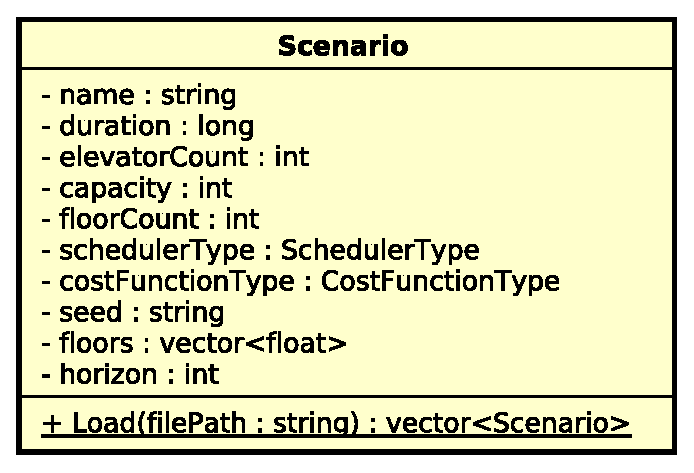
\includegraphics[scale=0.6]{img/Scenario}
  \caption{Diagrama de classes dos \textit{cenários}.}
\label{fig:diagram:scenario}
\end{figure}

\section{\label{model:events}Eventos}

A simulação de eventos discretos, como o próprio nome já diz, é orientada a
eventos. Isso significa dizer que as alterações no estado do sistema ocorrerão
somente na ocasião de algum evento e é preciso ser possível representar um
evento no contexto do simulador. Um evento é uma estrutura que deve possuir as
seguintes informações: (1) um número identificador; (2) o horário agendado para
a ocorrência do evento; (3) o tipo do evento.

Existem dois tipos de eventos que podem ocorrer durante uma simulação:

\begin{description}
  \item[Chegada de cliente] Um cliente chegou na fila de um andar.

  \item[Fim da simulação] A simulação atingiu a duração
especificada.\footnote{Este evento não necessariamente implica no fim imediato
da simulação, apenas que a chegada de novos clientes não ocorrerá mais. O
simulador ainda irá processar os clientes que estiverem nos andares ou dentro de
elevadores.}

\end{description}

Para obter tal funcionalidade foram criadas a classe abstrata \texttt{Event} e
as classes concretas que a especializam, representando os eventos de
\textbf{chegada de cliente} e \textbf{fim da simulação}, respectivamente:
\texttt{ClientArrival} e \texttt{FinishSimulation}
(figura~\ref{fig:diagram:events}).

\begin{figure}[htb!]
  \centering
  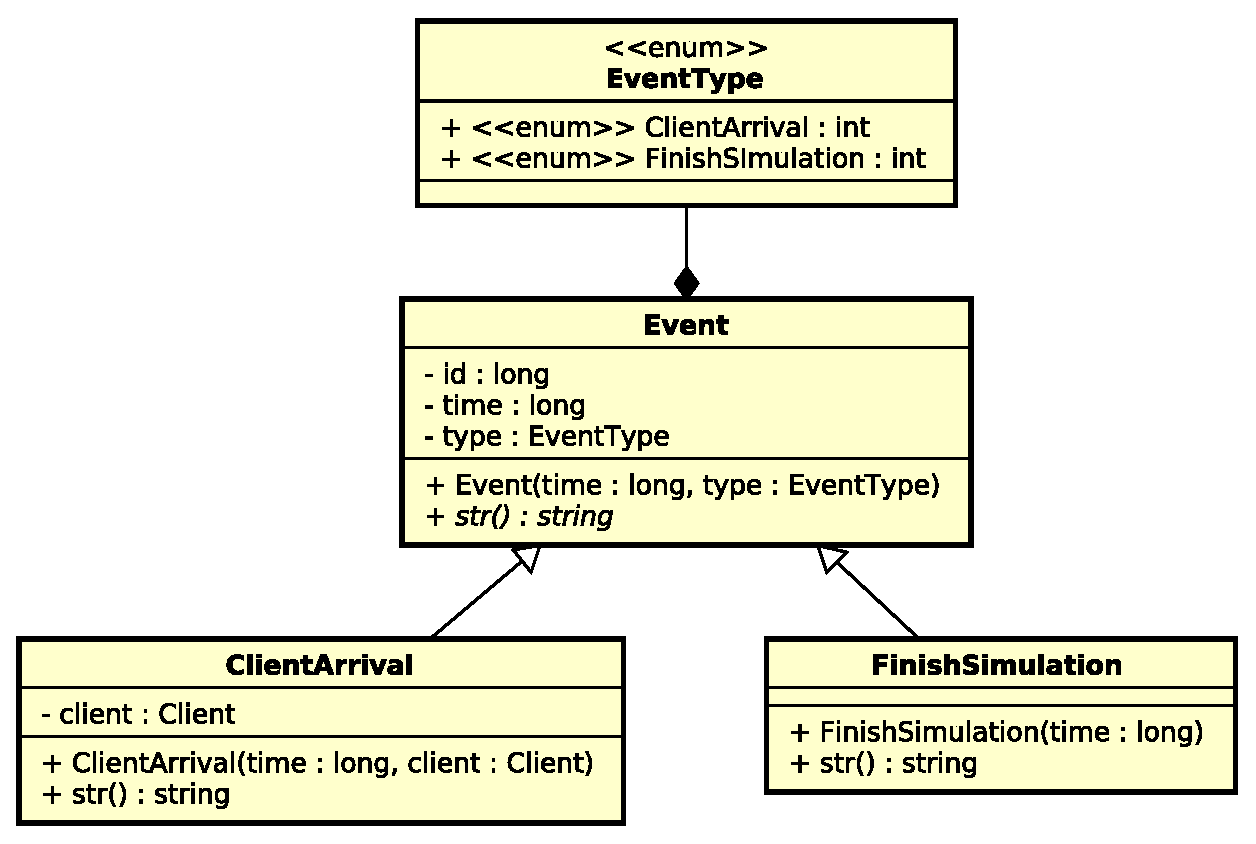
\includegraphics[scale=0.6]{img/Events}
  \caption{Diagrama de classes dos \textit{eventos e seus derivados}.}
\label{fig:diagram:events}
\end{figure}

\begin{description}
  \item[Event] \hfill \\
    Evento base composto pelo conjunto básico de informações para um evento.

    \begin{description}[leftmargin=!,labelwidth=\widthof{\bfseries client}]
      \item[\texttt{id}] Número identificador do evento.
      \item[\texttt{time}] Horário de ocorrência do evento.
      \item[\texttt{type}] Tipo do evento.
    \end{description}

  \item[ClientArrival] \hfill \\
    Evento especializado do tipo \textbf{chegada de cliente}. Contém,
    adicionalmente, as informações do cliente.

    \begin{description}[leftmargin=!,labelwidth=\widthof{\bfseries client}]
      \item[\texttt{client}] Cliente que gerou o evento.\footnote{Tipo complexo armazenando diversas informações sobre o cliente. \unsure{Colocar referência.}}
    \end{description}

  \item[FinishSimulation] \hfill \\
    Evento especializado do tipo \textbf{fim da simulação}. Não é necessária
    nenhuma informação adicional.
\end{description}

\section{\label{sec:model:event}Gerenciamento de eventos}

Na seção~\ref{simulator:flow} foram apresentados os componentes de um simulador.
Alguns destes componentes devem reagir na ocorrência de um evento, alterando o
seu estado interno de acordo com o tipo de evento ocorrido e as informações que
ele carrega consigo. Porém restam as questões de como saber qual evento será o
próximo a ocorrer e como notificar os elementos reativos disso. Portanto,
precisamos de mecanismos para criar e ordenar eventos e notificar os componentes
da ocorrência de um evento.

\subsection{Criação}

Não é possível prever em qual andar e qual momento um cliente irá chegar ao
prédio, tampouco qual o destino desejado por ele. Portanto, é correto afirmar
que a chegada de clientes em um prédio é um processo estocástico.

\begin{description}

\item[Horário de chegada] \hfill \\
Segundo~\cite{Ross:2006:IPM:1197141}, a taxa de chegada de clientes é um
processo de Poisson, com razão $\lambda$. Ou seja, o tempo entre novos clientes
são variáveis independentes, com valor esperado $\frac{1}{\lambda}$. Pode-se ver
na figura~\ref{fig:distribution:poisson} um exemplo de diferentes valores de
$\lambda$ gerando diferentes distribuições.

\begin{figure}[htb!]
  \centering
  \includegraphics[scale=1.0]{img/poisson.eps}
  \caption{Exemplos de distribuições de Poisson.}
\label{fig:distribution:poisson}
\end{figure}

Em um prédio no mundo real, esta distribuição varia de acordo com a hora do dia.
Por exemplo, nos horários do início do turno da manhã e no início do turno da
tarde, muito mais passageiros chegam ao térreo, com destino ao andar onde
trabalham. Para fim de simplificação, esta variação ao longo do dia não foi
considerada neste estudo. Conforme visto na seção \ref{model:scenario}, cada
andar do prédio possui um valor para $\lambda$, que permanece constante no
decorrer de toda a simulação.

\item[Andar de destino] \hfill \\
Já a probabilidade de um cliente ir de um andar para outro, em um tráfego
chamado de \textit{interfloor}, é um processo de Markov, com distribuições
normais (\textit{i.e.} uma média e um desvio padrão) que variam de acordo com a
hora do dia. Para fim de simplificação, esta variação ao longo do dia não foi
considerada neste estudo. Além disso, considera-se que a probabilidade de um
cliente ir para qualquer andar é a mesma - com exceção do próprio em que se
encontra, que é nula. Abaixo uma matriz de probabilidades para um prédio com 3
andares, representada por uma cadeia de Markov na figura
\ref{fig:distribution:markov}.

\[
  \begin{bmatrix}
    f_{11} & f_{12} & f_{13}  \\
    f_{21} & f_{22} & f_{23}  \\
    f_{31} & f_{32} & f_{33}
  \end{bmatrix} = \begin{bmatrix}
    0.0 & 0.5 & 0.5  \\
    0.5 & 0.0 & 0.5  \\
    0.5 & 0.5 & 0.0
  \end{bmatrix}
\]

\begin{figure}[htb!]
  \centering
  \includegraphics[scale=0.4]{img/markov.eps}
  \caption{Exemplo de cadeia de Markov para um prédio de 3 andares.}
\label{fig:distribution:markov}
\end{figure}

\item[EventFactory] \hfill \\
A classe \texttt{EventFactory}, ou \textit{fábrica de eventos}, foi criada para
ser uma unidade de coesão ao criar chegadas de clientes no prédio. Cada andar do
prédio possui uma instância desta classe. Seus componentes são:

  \begin{description}[leftmargin=!,labelwidth=\widthof{\bfseries hasNextEvent}]
    \item[\texttt{clock}] Referência para o relógio da simulação.
    \item[\texttt{floor}] Referência para o andar daquele \texttt{EventFactory}.
    \item[\texttt{random engine}] Gerador de números aleatórios.
    \item[\texttt{destination}] Distribuição Discreta, utilizada para sortear andares de destino.
    \item[\texttt{arrival}] Distribuição de Poisson, utilizada para sortear horários de eventos futuros.
  \end{description}

  O algoritmo \ref{alg:eventcreation} ilustra a criação de um novo evento.
  Primeiro, o método \texttt{CreateFutureArrival} calcula o horário do novo
  evento. Isto é feito somando-se o horário atual do \textit{relógio da
  simulação} com um tempo sorteado pela distribuição de Poisson específica
  daquele andar. Na sequência, é sorteado o andar destino pela distribuição
  discreta também específica do andar. Feito isso, é criado um novo evento do
  tipo \textbf{chegada de cliente} com as informações sorteadas e tendo como
  origem o andar atual. No fim, o evento criado é adicionado à fila de eventos
  (seção \ref{model:queue}).

  \begin{algorithm}[htb]
  \begin{center}
  \begin{algorithmic}[1]
  \Function{EventFactory::CreateFutureArrival}{$eventQueue, clock, floor, randomEngine$}
    \State $eventTime \leftarrow clock.\Call{currentTime}{}() + \Call{getNextTime}{randomEngine}$
    \State $destination \leftarrow \Call{getNextDestination}{randomEngine}$
    \State $clientArrival \leftarrow \Call{ClientArrival}{floor, destination, eventTime}$
    \State $eventQueue.\Call{push}{clientArrival}$
  \EndFunction
  \State
  \Function{EventFactory::GetNextTime}{$randomEngine$}
    \State \textbf{return} $arrival(randomEngine)$
  \EndFunction
  \State
  \Function{EventFactory::GetNextDestination}{$randomEngine$}
    \State \textbf{return} $destination(randomEngine)$
  \EndFunction
  \end{algorithmic}
  \end{center}
  \caption{\label{alg:eventcreation}Criação de um novo \textit{evento de chegada de cliente}.}
  \end{algorithm}
\end{description}

\subsection{Priorização} \label{model:queue}

Na seção~\ref{simulator:movation:discrete} foi apresentado o \textit{mecanismo
de avanço de tempo para o próximo evento}, onde deve-se verificar, em uma lista
de eventos, qual é o próximo evento a ocorrer. Dado um conjunto de eventos
agendados (ou seja, ainda não ocorridos), o primeiro evento a ocorrer é
justamente o que possui o menor tempo de agendamento. Um tipo abstrato de dados
que serve para este propósito é uma \textit{fila prioritária}, ou
\textit{priority queue}, que funciona de forma similar a filas \textit{FIFO},
com a diferença de que cada elemento armazenado possui uma prioridade associada.
A \textit{fila prioritária}, implementada na classe \texttt{EventQueue}, irá
atender os elementos por ordem de prioridade, da maior para a menor. Ao
considerar que a prioridade de um evento é inversamente proporcional ao instante
em que irá ocorrer - ou seja, quanto menor o tempo do evento maior é a sua
prioridade -, temos uma fila na qual o próximo elemento a ser atendido sempre
será o próximo evento a ocorrer.

\begin{description}
  \item[EventQueue] \hfill \\
    Encapsula uma fila prioritária de eventos. Adicionalmente, utiliza a classe
    \texttt{EventComparator}, que implementa a relação de ordem entre os
    eventos.

    \begin{description}[leftmargin=!,labelwidth=\widthof{\bfseries hasNextEvent}]
      \item[\texttt{push}] Insere um evento na fila.
      \item[\texttt{top}] Recupera o primeiro evento da fila.
      \item[\texttt{pop}] Remove o primeiro evento da fila.
      \item[\texttt{hasNextEvent}] Verifica se a fila possui eventos.
    \end{description}
\end{description}

\begin{figure}[htb!]
  \centering
  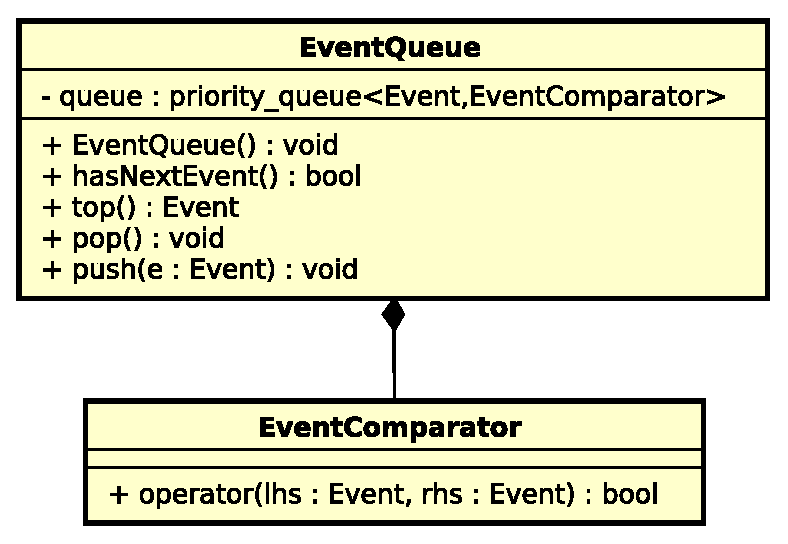
\includegraphics[scale=0.6]{img/EventQueue}
  \caption{Diagrama de classes da \textit{criação e priorização de eventos}.}
\label{fig:diagram:event:manage}
\end{figure}

\subsection{Notificação}

Quando o próximo evento a ocorrer é conhecido, o problema passa a ser notificar
os elementos reativos que este evento ocorreu para que os mesmos possam
atualizar seus estados internos. De acordo com Gamma
\cite{Gamma:1995:DPE:186897}, o padrão \textit{Observer} é um \textit{design
pattern} indicado para resolver este problema. Este \textit{pattern} define uma
dependência de um-para-muitos ($1:N$) entre objetos de modo que, quando este um
objeto (\textit{subject}) tem seu estado alterado, todos os seus dependentes
(\textit{observers}) são notificados deste mudança. Por consequência, estes
dependentes podem modificar seu estado interno baseando-se nas informações desta
notificação.

Este padrão foi utilizado para implementar a funcionalidade de notificação de
eventos, ilustrado no diagrama da figura~\ref{fig:diagram:notification}. Para
isto, foram criados os seguintes componentes:

\begin{figure}[htb!]
  \centering
  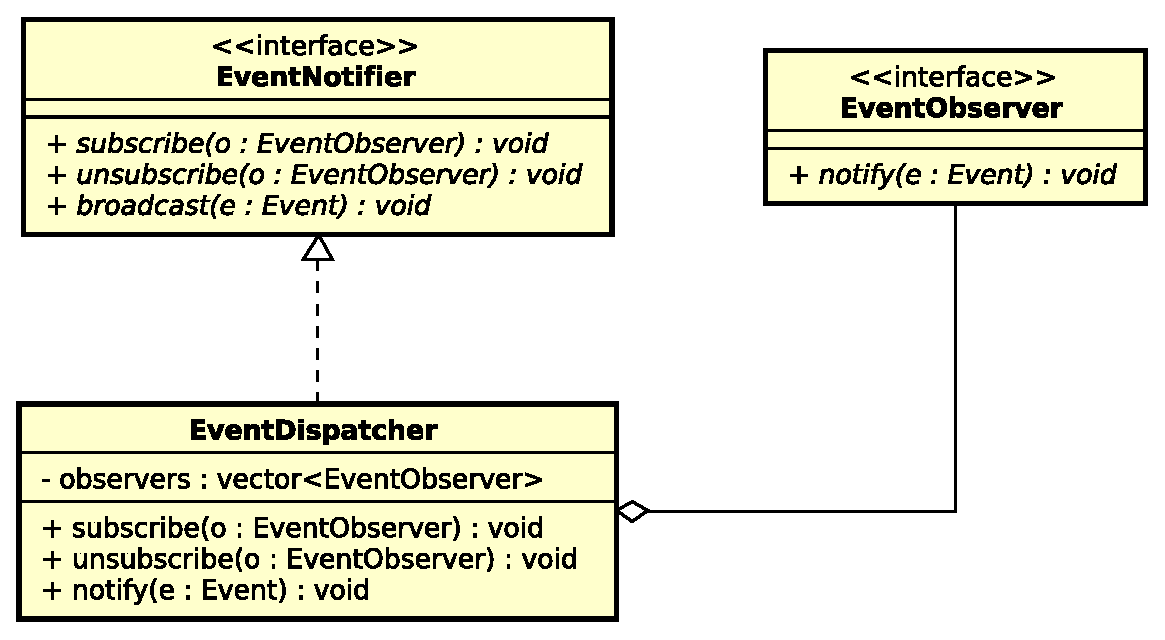
\includegraphics[scale=0.6]{img/EventNotifier}
  \caption{Diagrama de classes da \textit{notificação de eventos}.}
\label{fig:diagram:notification}
\end{figure}

\begin{description}
  \item[EventObserver] \hfill \\
    Classe abstrata a ser realizada por qualquer outra classe que deseje receber
    notificações de eventos. Possui um único método abstrato.

    \begin{description}[leftmargin=!,labelwidth=\widthof{\bfseries unsubscribe}]
      \item[\texttt{notify}] Recebe a notificação da ocorrência de um evento.
    \end{description}

  \item[EventNotifier] \hfill \\
    Classe abstrata a ser realizada por qualquer outra classe que deseje
    notificar a ocorrência de eventos. Define métodos para que objetos que
    implementem a classe abstrata \textit{EventObserver} possam registrar-se
    para receber notificações de ocorrências de eventos. Seus métodos abstratos
    são:

    \begin{description}[leftmargin=!,labelwidth=\widthof{\bfseries unsubscribe}]
      \item[\texttt{subscribe}] Adiciona um \textit{observer}.
      \item[\texttt{unsubscribe}] Remove um \textit{observer}.
      \item[\texttt{broadcast}] Notifica todos os \textit{observers} registrados da ocorrência de um evento.
    \end{description}

  \item[EventDispatcher] \hfill \\
    Classe concreta que realiza a interface \texttt{EventNotifier}. Possui uma
    estrutura de dados para armazenar quais \textit{observers} se registraram
    através dos métodos \texttt{subscribe} e \texttt{unsubscribe}.
\end{description}

Três importantes componentes do simulador podem se beneficiar desta construção:
(1) o \textit{relógio do sistema} (classe \texttt{Clock}); (2) os
\textit{contadores estatísticos} (classe \texttt{Statistics}); e (3) o
\textit{estado do sistema} (classe \texttt{Building}). Na ocorrência de um
evento, estas três entidades devem ser notificadas e cada uma irá alterar seu
estado interno da forma adequada. Para isto, devem implementar a interface
\texttt{EventObserver} e registrarem-se no \texttt{EventDispatcher}. Assim, o
\texttt{EventDispatcher} e a \texttt{EventQueue} podem, juntos, notificar aos
componentes reativos exatamente qual evento ocorreu em cada iteração da
simulação, na ordem correta dos eventos.

\section{\label{model:reactive}Componentes reativos}

Durante a execução da simulação, à medida que eventos ocorrem, componentes do
simulador devem alterar seu estado interno de acordo com o evento ocorrido,
levando o estado do simulador a uma nova situação. A seguir são apresentadas as
classes que representam estes componentes no simulador.

\subsection{Estado do sistema}

Entre os componentes fundamentais de um simulador destaca-se a representação do
\textit{estado do sistema}, uma coleção de variáveis necessárias para descrever
o sistema em um instante em particular da simulação~\cite{Law}. Neste projeto, a
classe \texttt{Building} é responsável por encapsular o conjunto de informações
que definem este estado (figura~\ref{fig:diagram:model}). Esta classe é
responsável por gerenciar múltiplas instâncias de elevadores (classe
\texttt{Elevator}), andares (classe \texttt{Floor}) e clientes (classe
\texttt{Client}) e relacionar estas instâncias entre si - reproduzindo, deste
modo, as dinâmicas do sistema do mundo real que está sendo simulado.

\begin{figure}[htb!]
  \centering
  \includegraphics[scale=0.6]{img/Model.eps}
  \caption{Diagrama de classes do \textit{estado do sistema}.}
\label{fig:diagram:model}
\end{figure}

\begin{description}
  \item[Floor] \hfill \\
    Parte componente de um prédio. Possui os seguintes atributos:

  \begin{description}[leftmargin=!,labelwidth=\widthof{\bfseries arrivalFloor}]
    \item[\texttt{number}] Número do andar em que a parada deve ser realizada.
    \item[\texttt{lambda}] Direção na qual a parada deve ser realizada.
    \item[\texttt{upLine}] Direção na qual a parada deve ser realizada.
    \item[\texttt{downLine}] Direção na qual a parada deve ser realizada.
    \item[\texttt{eventFactory}] Direção na qual a parada deve ser realizada.
  \end{description}

     possuindo uma numeração e duas
    filas\footnote{No mundo real, apesar de aparentemente as pessoas formarem
    uma fila única, os membros da fila respeitam o sentido de viagem do elevador
    e implicitamente separam-se em duas filas: uma para subir e outra para
    descer.}: uma para clientes que desejam descer e outra para clientes que
    desejam subir.

\item[Call] \hfill \\
  Representa uma parada a ser realizada por algum elevador. É composta pelos seguintes
  atributos:

  \begin{description}[leftmargin=!,labelwidth=\widthof{\bfseries arrivalFloor}]
    \item[\texttt{number}] Número do andar em que a parada deve ser realizada.
    \item[\texttt{direction}] Direção na qual a parada deve ser realizada.
  \end{description}

  Por exemplo, pode existir uma parada no andar 8 para subir; uma parada no andar
  4 para descer; etc.

\item[Elevator] \hfill \\
  Representa um elevador. Possui os seguintes atributos:

  \begin{description}[leftmargin=!,labelwidth=\widthof{\bfseries arrivalFloor}]
    \item[\texttt{number}] Número identificador do elevador.
    \item[\texttt{capacity}] Capacidade máxima do elevador (em número de clientes).
    \item[\texttt{location}] Número do andar no qual o elevador se encontra.
    \item[\texttt{destination}] Chamada destino do elevador (classe \texttt{Call}).
    \item[\texttt{status}] Situação atual do elevador: \textit{moving} (movendo-se) ou \textit{idle} (ocioso).
    \item[\texttt{direction}] Direção na qual o elevador está se movendo (no caso de não estar ocioso).
    \item[\texttt{passengers}] Conjunto com os passageiros que embarcaram no elevador e ainda não desembarcaram.
  \end{description}

\item[Client] \hfill \\
  Representa uma pessoa que chegou a um andar e deseja se dirigir a outro andar.
  Possui os seguintes atributos:

  \begin{description}[leftmargin=!,labelwidth=\widthof{\bfseries arrivalFloor}]
    \item[\texttt{id}] Número identificador do cliente.
    \item[\texttt{destination}] Número do andar ao qual o cliente deseja dirigir-se.
    \item[\texttt{arrivalFloor}] Número do andar no qual o cliente chegou.
    \item[\texttt{createTime}] Horário em que o cliente chegou ao prédio.
    \item[\texttt{pickupTime}] Horário em que o cliente embarcou em um elevador.
  \end{description}

  \item[Building] \hfill \\
    Representa a composição do prédio sendo simulado. Possui um conjunto de
    elevadores, uma lista ordenada de andares e um método \texttt{reset},
    utilizado para a inicialização da simulação. Um prédio é formado por no
    mínimo um elevador e no mínimo um andar\footnote{Isto em termos conceituais;
    porém, não há sentido na existência de um sistema de elevadores em uma
    edificação com somente um andar. De fato, conforme afirmado na
    seção~\ref{section:scenarios}, serão simulados prédios com, no mínimo, 4
    andares.}.

\end{description}

\subsection{Relógio da simulação}

O \textit{relógio da simulação} é representado pela classe \texttt{Clock}
(figura~\ref{fig:diagram:clock}). Esta classe encapsula o atributo privado
\texttt{time} e provê métodos para sua consulta e atualização.

\begin{figure}[htb!]
  \centering
  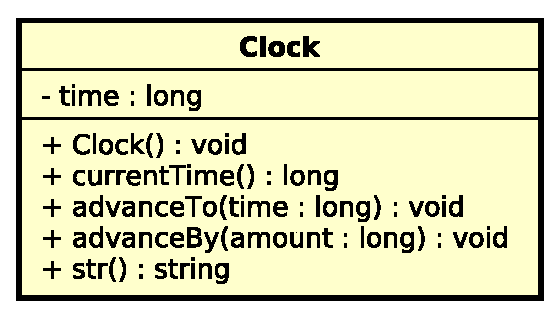
\includegraphics[scale=0.6]{img/Clock}
  \caption{Diagrama de classes do \textit{relógio do sistema}.}
\label{fig:diagram:clock}
\end{figure}

\begin{description}[leftmargin=!,labelwidth=\widthof{\bfseries currentTime}]
  \item[\texttt{currentTime}] Retorna o horário atual do \textit{relógio da simulação}.
  \item[\texttt{advanceTo}] Avança o \textit{relógio da simulação} para um horário arbitrário.
  \item[\texttt{advanceBy}] Avança o \textit{relógio da simulação} em uma quantidade arbitrária de segundos.
  \item[\texttt{str}] Representação textual do \textit{relógio da simulação} (utilizado em \textit{logs}).
  \item[\texttt{notify}]
  Realização da classe abstrata \texttt{EventObserver}. Ao ser notificado de um
  evento, o \textit{relógio da simulação} deve avançar o relógio interno para o
  instante da ocorrência do evento, independentemente do tipo de evento que
  ocorreu. O algoritmo \ref{alg:advanceto} ilustra este conceito.
\end{description}

\begin{algorithm}[htb]
\begin{center}
\begin{algorithmic}[1]
\Function{Clock::Notify}{$event$}
  \State $eventTime \leftarrow event.\Call{getTime}{}$
  \State \Call{advanceTo}{$eventTime$}
\EndFunction
\end{algorithmic}
\end{center}
\caption{\label{alg:advanceto}\textit{Relógio do sistema} reagindo a um evento.}
\end{algorithm}

\subsection{Contadores estatísticos}

Os \textit{contadores estatísticos} da simulação são responsáveis por coletar e
sumarizar dados do sistema durante toda a execução da simulação. Sua existência
permite a realização de análises qualitativas e quantitativas a respeito do
sistema simulado. Neste projeto, os \textit{contadores estatísticos} são
representados pelas estruturas \texttt{Arrival} e \texttt{Trip} e pela classe
\texttt{Statistics} (figura~\ref{fig:diagram:statistics}).

\begin{figure}[htb!]
  \centering
  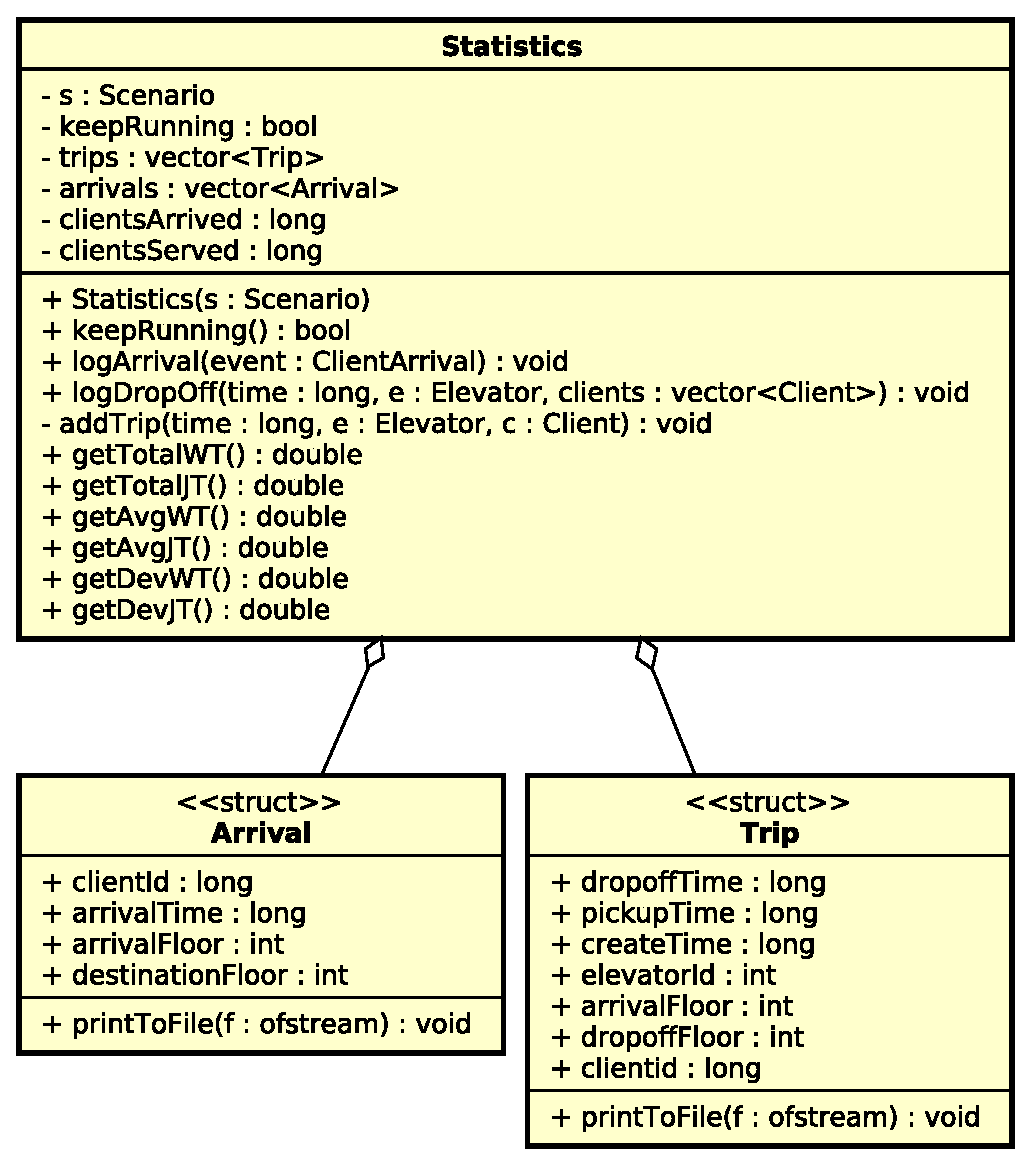
\includegraphics[scale=0.6]{img/Statistics}
  \caption{Diagrama de classes dos \textit{contadores estatísticos}.}
\label{fig:diagram:statistics}
\end{figure}

\begin{description}
  \item[Arrival] \hfill \\
    Uma instância desta estrutura armazena informações coletadas quando um
    cliente chega ao prédio. Tais informações são:

    \begin{description}[leftmargin=!,labelwidth=\widthof{\bfseries destinationFloor}]
      \item[\texttt{clientId}] Número identificador do cliente.
      \item[\texttt{arrivalTime}] Horário em que o cliente chegou ao prédio.
      \item[\texttt{arrivalFloor}] Número do andar no qual o cliente chegou.
      \item[\texttt{destinationFloor}] Andar de destino ao qual o cliente deseja dirigir-se.
    \end{description}

  \item[Trip] \hfill \\
    Uma instância desta estrutura armazena informações coletadas quando um
    cliente desembarca de um elevador. Tais informações são:

    \begin{description}[leftmargin=!,labelwidth=\widthof{\bfseries destinationFloor}]
      \item[\texttt{clientId}] Número identificador do cliente.
      \item[\texttt{dropoffTime}] Horário em que o cliente desembarcou do elevador.
      \item[\texttt{createTime}] Horário em que o cliente chegou ao prédio.
      \item[\texttt{elevatorId}] Número do elevador do qual o cliente desembarcou.
      \item[\texttt{arrivalFloor}] Número do andar no qual o cliente chegou.
      \item[\texttt{dropoffFloor}] Número do andar no qual o cliente desembarcou.
    \end{description}

  \item[Statistics] \hfill \\
    Armazena as estatísticas coletadas durante a simulação e fornece cálculos
    estatísticos sobre o volume de dados coletados no fim da simulação. Seus
    métodos são:

    \begin{description}[leftmargin=!,labelwidth=\widthof{\bfseries destinationFloor}]
      \item[\texttt{logDropOff}] Registra a ocorrência de um desembarque.
      \item[\texttt{logTrip}] Registra a ocorrência de uma chegada de um cliente.
      \item[\texttt{getAvgWT}] Calcula o tempo de espera médio.
      \item[\texttt{getDevWt}] Calculo o desvio padrão do tempo de espera.
      \item[\texttt{getTotalWT}] Calcula o tempo de espera total.
      \item[\texttt{getAvgWT}] Calcula o tempo de jornada médio.
      \item[\texttt{getDevWt}] Calcula o desvio padrão do tempo de jornada.
      \item[\texttt{getTotalWT}] Calcula o tempo de jornada total.
      \item[\texttt{keepRunning}] Avalia se a simulação deve terminar\footnote{por exemplo, se o tempo de duração da simulação já se passou.}.
      \item[\texttt{notify}]
        Realização da classe abstrata \texttt{EventObserver}. Ao ser notificado
        de um evento: se for do tipo \textbf{chegada de cliente}, deve coletar e
        armazenar as informações desta nova chegada; se for do tipo \textbf{fim
        da simulação}, deve altera o estado do atributo privado
        \texttt{keepRunning} para \texttt{false}. Esta ação irá interromper a
        chegada de novos clientes. O algoritmo \ref{alg:statistics} ilustra este
        conceito.
    \end{description}
\end{description}

\begin{algorithm}[htb]
\begin{center}
\begin{algorithmic}[1]
\Function{Statistics::Notify}{$event$}
  \If{$event.$\Call{getType}{} $= ClientArrival$}
    \State \Call{logArrival}{$event$}
  \ElsIf{$event.$\Call{getType}{} $= FinishSimulation$}
    \State $keepRunning \leftarrow false$
  \EndIf
\EndFunction
\end{algorithmic}
\end{center}
\caption{\label{alg:statistics}\textit{Contadores estatísticos} reagindo a um evento.}
\end{algorithm}

  % if (event->getType() == EventType::clientArrival) {
  %   logArrival(std::static_pointer_cast<const ClientArrival>(event));
  % }

  % if (event->getType() == EventType::finishSimulation) {
  %   _keepRunning = false;
  % }

\section{\label{model:simulador}Simulador}

\unsure{Aqui mostrar como o simulador cola todas estas partes e faz funcionar.}

\section{\label{model:schedulers}Algoritmos de Agendamento}
Neste trabalho, dois algoritmos de agendamento foram implementados, o
\textit{Simple Scheduler} (seção~\ref{model:schedulers:simple}) e o
\textit{Planning Scheduler} (seção~\ref{model:schedulers:planning}).

Ambos algoritmos são implementados em classes próprias, que herdam de uma classe
\texttt{Scheduler}. Este relacionamento pode ser visto mais claramente na
figura~\ref{fig:model:schedulers:uml:base}.

\begin{figure}[htb]
  \centering
  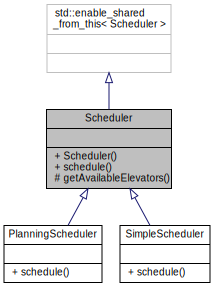
\includegraphics{doc/latex/class_scheduler__inherit__graph}
  \caption{Diagrama UML das classes Scheduler}
  \label{fig:model:schedulers:uml:base}
\end{figure}

Os \textit{schedulers} têm apenas um método público, chamado \texttt{int
  schedule()}, que recebe como parâmetro a função de custo e um ponteiro para o
prédio, além de, opcionalmente, um elevador para ser excluído.

\unsure{Onde falamos de por que é importante excluir elevadores do schedule às
  vezes? (Vanzella)}
Excluir um elevador é importante, como foi falado na Sessão XXX. Há um método
protegido na classe \texttt{Scheduler}, chamado
\texttt{getAvailableElevators()}, que retorna uma lista de elevadores, excluindo
aqueles que não podem ser utilizados.

\subsection{\label{model:schedulers:simple}Simple}
O \textit{Simple Scheduler}, como o nome sugere, tem um comportamento bem
simples: itera pela lista de elevadores disponíveis, calculando a função de
custo para cada um, e retorna o de menor custo.

\subsection{\label{model:schedulers:planning}Planning}
\lipsum[5]

\section{\label{model:costfunctions}Algoritmos de Função de Custo}
As funções de custo herdam de uma classe base, chamada \texttt{CostFunction},
que possui apenas um método público, \texttt{float calculate()}, que retorna o
valor da função para aquela combinação entre o elevador e o cliente.

Isto pode ser visto em mais detalhes na figura~\ref{fig:model:costfunction:uml:base}.

\begin{figure}[htb]
  \centering
  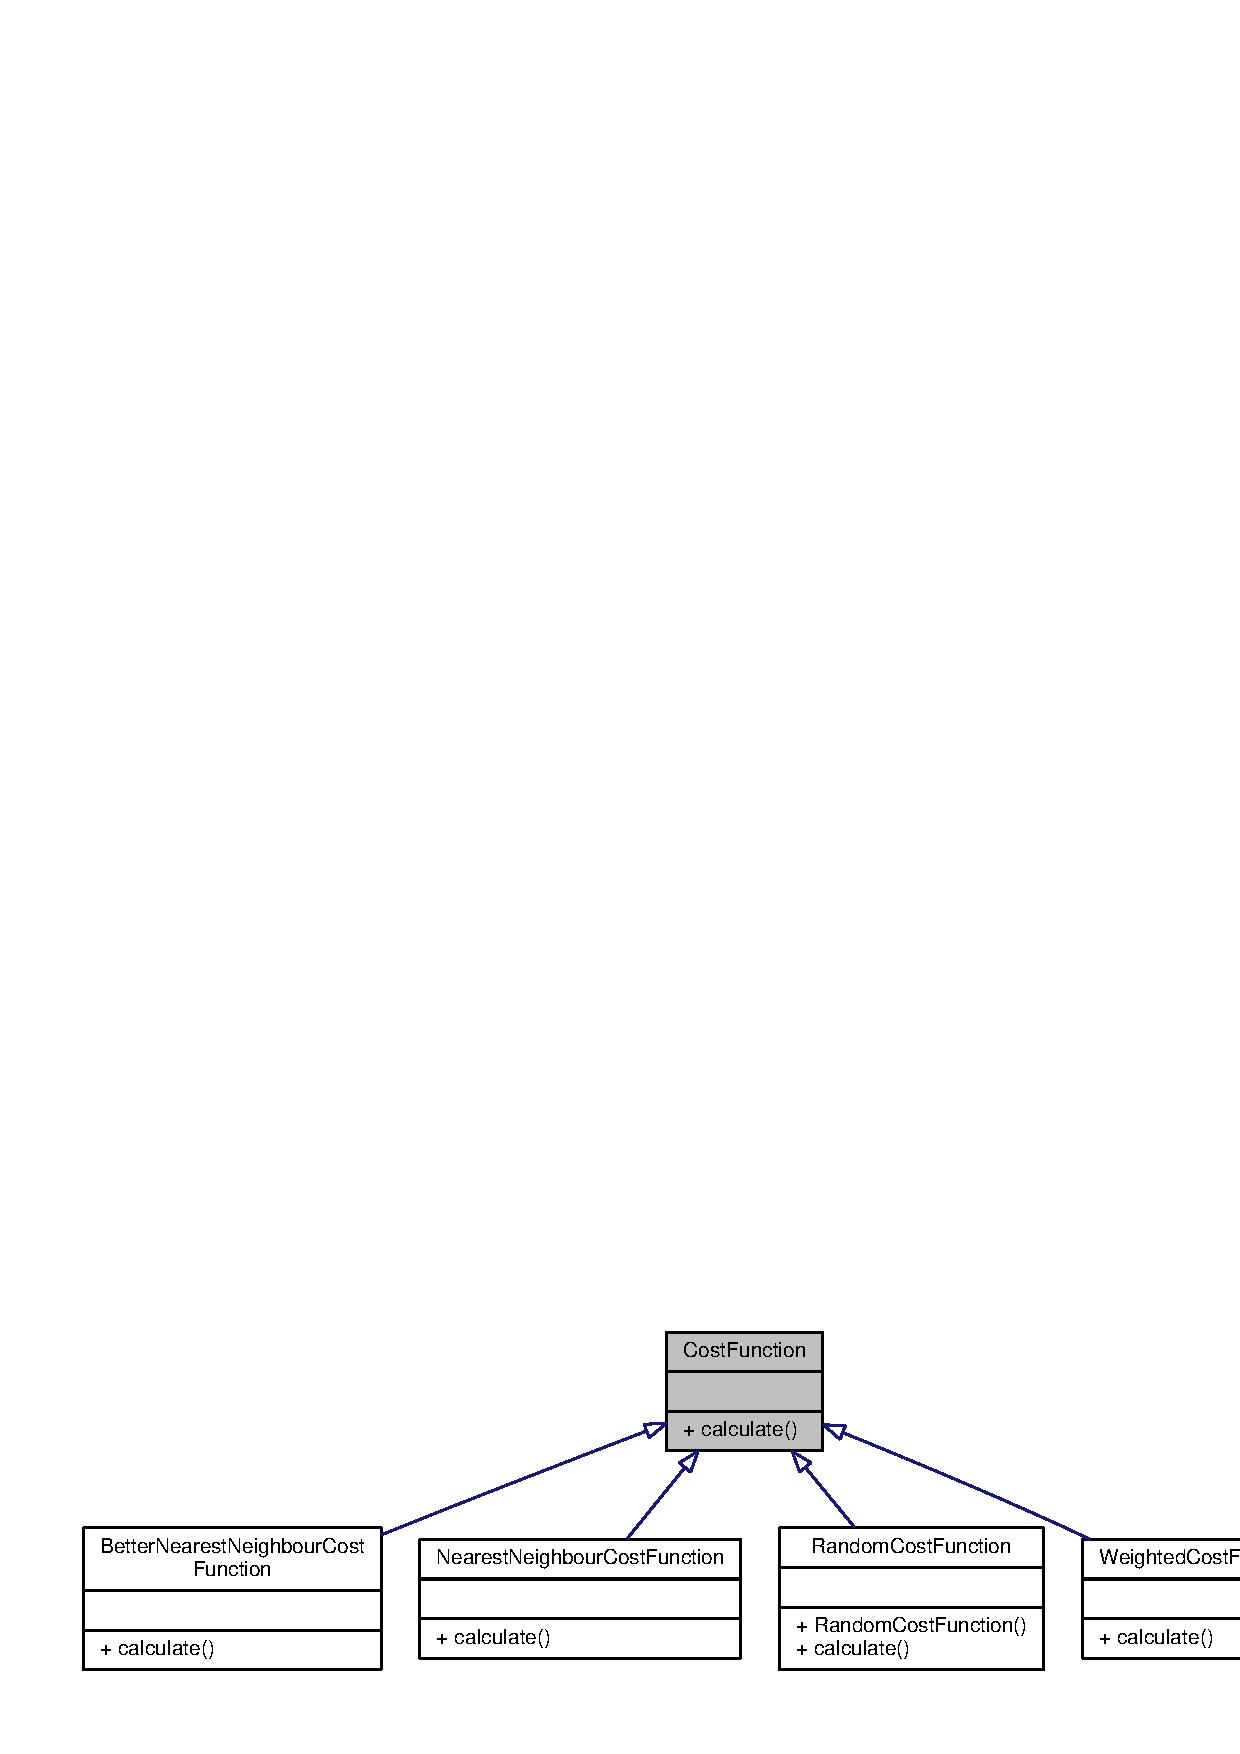
\includegraphics[scale=0.8]{doc/latex/class_cost_function__inherit__graph}
  \caption{Diagrama UML das classes CostFunction}
  \label{fig:model:costfunction:uml:base}
\end{figure}

\subsection{\label{model:costfunctions:random}Random}
A Função de Custo \textit{Random} serve como base de comparação para as demais.
Ela retorna um valor aleatório entre zero e um cada vez que for chamada, e,
portanto, deve resultar em um agendamento pior do que qualquer alternativa.

Olhando-se a figura~\ref{fig:model:costfunction:uml:base}, nota-se que ela é a
única função de custo com um construtor. Isto se dá por que é necessário
inicializar-se a geração de números aleatórios, de modo a gerar estes números de
forma consistente.
\unsure{Vale a pena colocar o código deste construtor aqui? (Vanzella)}

\subsection{\label{model:costfunctions:nn}Nearest Neighbour}
Esta função de custo retorna, como custo, a distância em valor absoluto do
elevador para o cliente. Ela ignora a direção na qual o elevador está viajando.

\unsure{Colocar o código aqui? Tem 2 linhas. (Vanzella)}

\subsection{\label{model:costfunctions:bnn}Better Nearest Neighbour}
A Função de Custo \textit{Better Nearest Neighbour} bonifica elevadores que
estão indo na direção do chamado, dividindo seu custo por $\sqrt 2$ e bonifica
mais ainda os elevadores parados, dividindo seu custo por $2$. O custo antes
deste bônus é calculado de maneira igual à \textit{Nearest Neighbour}.

\subsection{\label{model:costfunctions:weighted}Weighted}
A Função \textit{Weighted} toma uma decisão diferente da \textit{Better Nearest
  Neighbour} para melhorar a \textit{Nearest Neighbour}. Em vez de bonificar
elevadores parados ou elevadores que estão indo na direção do cliente, esta
função bonifica elevadores mais vazios, dividindo o custo (que é a distância
entre o cliente e o elevador) pela ocupação do elevador.\footnote{Como foi visto
na Sessão~XXX, podemos inferir a ocupação pela balança interna do elevador, em
alguns cenários reais.}
\unsure{Sessão XXX (Vanzella)}

\section{\label{model:report}Geração de Relatórios}
\lipsum[5]

\dirtree{%
.1 output.
.2 High-rise\DTcomment{Nome do cenário.}.
.3 1 Simple Random\DTcomment{Diretório da estratégia.}.
.4 run.log\DTcomment{Log de execução da estratégia.}.
.4 report.log\DTcomment{Relatório das métricas da estratégia.}.
.4 trips.log\DTcomment{Arquivo CSV contendo os desembarques.}.
.3 2 Simple NearestNeighbour.
.4 run.log.
.4 report.log.
.4 trips.log.
.3 3 Simple BetterNearestNeighbour.
.4 run.log.
.4 report.log.
.4 trips.log.
.3 4 Simple Weighted.
.4 run.log.
.4 report.log.
.4 trips.log.
.3 5 Planning.
.4 run.log.
.4 report.log.
.4 trips.log.
.3 arrivals.log\DTcomment{Arquivo CSV contendo as chegadas de clientes no prédio.}.
.3 report.log\DTcomment{Relatório unificado de todas as estratégias do cenário.}.
}

\subsection{\label{model:report:charts}Geração de Gráficos}
\lipsum[5]
\chapter{\label{chap:results}Resultados}

\section{Cenário \textit{Low-rise}}

\lipsum[1]

\begin{table}[htb!]
\centering
\caption{Parâmetros do cenário \textit{Low-rise}.}
\label{tab:results:lowrise:params}
\begin{tabular}{|r|l|}
\hline
\textbf{Propriedade}          & \textbf{Valor}       \\ \hline
\textit{Nome}                 & Low-rise             \\ \hline
\textit{Duração (s)}          & 43200                \\ \hline
\textit{Semente}              & 54TH7hboAG1iOsDIDhJp \\ \hline
\textit{Elevatores}           & 2                    \\ \hline
\textit{Capacidade}           & 6                    \\ \hline
\textit{Andares}              & 11                   \\ \hline
\textit{Horizonte (planning)} & 5                    \\ \hline
\end{tabular}
\end{table}

\begin{table}[htb!]
\centering
\caption{Resultados obtidos da simulação do cenário \textit{Low-rise}.}
\label{tab:results:lowrise}
\begin{tabular}{|c|c|r|r|r|r|r|r|}
\hline
\multicolumn{2}{|c|}{\textbf{}}                 & \multicolumn{3}{c|}{\textbf{Tempo de Espera}}                                                                    & \multicolumn{3}{c|}{\textbf{Tempo de Jornada}}                                                                                                                       \\ \hline
\textbf{Agendamento} & \textbf{Função de Custo} & \multicolumn{1}{c|}{\textit{Médio}} & \multicolumn{1}{c|}{\textit{Desvio}} & \multicolumn{1}{c|}{\textit{Total}} & \multicolumn{1}{c|}{\textit{Médio}}                   & \multicolumn{1}{c|}{\textit{Desvio}}                  & \multicolumn{1}{c|}{\textit{Total}}                  \\ \hline
\textit{Simple}      & \textit{Random}          & \cellcolor[HTML]{FD6864}5.4064      & \cellcolor[HTML]{FD6864}4.1792       & \cellcolor[HTML]{FD6864}16933       & \cellcolor[HTML]{FD6864}{\color[HTML]{000000} 4.4949} & 2.8676                                                & \cellcolor[HTML]{FD6864}{\color[HTML]{000000} 14078} \\ \hline
\textit{Planning}    & \textit{Random}          & \cellcolor[HTML]{67FD9A}3.1580      & \cellcolor[HTML]{67FD9A}2.8688       & \cellcolor[HTML]{67FD9A}9891        & 4.4713                                                & \cellcolor[HTML]{FD6864}{\color[HTML]{000000} 3.0005} & 14004                                                \\ \hline
\textit{Simple}      & \textit{NN}              & 3.5144                              & \cellcolor[HTML]{FFFFFF}3.5768       & 11007                               & 4.4700                                                & 2.8565                                                & 14000                                                \\ \hline
\textit{Planning}    & \textit{NN}              & 3.2273                              & 3.0515                               & 10108                               & 4.4770                                                & 2.9796                                                & 14022                                                \\ \hline
\textit{Simple}      & \textit{BNN}             & 3.3547                              & 3.2931                               & 10507                               & 4.4674                                                & 2.9163                                                & 13992                                                \\ \hline
\textit{Planning}    & \textit{BNN}             & 3.1830                              & 2.9150                               & 9969                                & \cellcolor[HTML]{67FD9A}4.4623                        & \cellcolor[HTML]{FFFFFF}2.9787                        & \cellcolor[HTML]{67FD9A}13976                        \\ \hline
\textit{Simple}      & \textit{Weighted}        & 3.7149                              & 3.8036                               & 11635                               & 4.4719                                                & \cellcolor[HTML]{67FD9A}2.7997                        & 14006                                                \\ \hline
\textit{Planning}    & \textit{Weighted}        & 3.2529                              & 3.0760                               & 10188                               & 4.4789                                                & 2.9714                                                & 14028                                                \\ \hline
\end{tabular}
\end{table}

\section{Cenário \textit{High-rise}}

\lipsum[1]

\begin{table}[htb!]
\centering
\caption{Parâmetros do cenário \textit{High-rise}.}
\label{tab:results:highrise:params}
\begin{tabular}{|r|l|}
\hline
\textbf{Propriedade}          & \textbf{Valor}       \\ \hline
\textit{Nome}                 & High-rise            \\ \hline
\textit{Duração (s)}          & 43200                \\ \hline
\textit{Semente}              & w9JwgykwejtoL2icSgHo \\ \hline
\textit{Elevatores}           & 8                    \\ \hline
\textit{Capacidade}           & 10                   \\ \hline
\textit{Andares}              & 39                   \\ \hline
\textit{Horizonte (planning)} & 2                    \\ \hline
\end{tabular}
\end{table}

\begin{table}[htb!]
\centering
\caption{Resultados obtidos da simulação do cenário \textit{High-rise}.}
\label{tab:results:highrise}
\begin{tabular}{|c|c|r|r|r|r|r|r|}
\hline
\multicolumn{2}{|c|}{\textbf{}}                 & \multicolumn{3}{c|}{\textbf{Tempo de Espera}}                                                                    & \multicolumn{3}{c|}{\textbf{Tempo de Jornada}}                                                                                                                       \\ \hline
\textbf{Agendamento} & \textbf{Função de Custo} & \multicolumn{1}{c|}{\textit{Médio}} & \multicolumn{1}{c|}{\textit{Desvio}} & \multicolumn{1}{c|}{\textit{Total}} & \multicolumn{1}{c|}{\textit{Médio}}                   & \multicolumn{1}{c|}{\textit{Desvio}}                  & \multicolumn{1}{c|}{\textit{Total}}                  \\ \hline
\textit{Simple}      & \textit{Random}          & 25.9981                         & 28.0464                         & 190124                          & 15.2595                         & 14.9190                         & 111593                          \\ \hline
\textit{Planning}    & \textit{Random}          &  8.8829                         & 16.5500                         &  64961                          & 15.1742                         & 12.0139                         & 110969                          \\ \hline
\textit{Simple}      & \textit{NN}              & 20.3395                         & 37.1902                         & 148743                          & 15.0993                         & 11.4479                         & 110421                          \\ \hline
\textit{Planning}    & \textit{NN}              &  9.9824                         & 19.4451                         &  73001                          & 15.1991                         & 11.4878                         & 111151                          \\ \hline
\textit{Simple}      & \textit{BNN}             & 13.5243                         & 23.5950                         &  98903                          & 15.0550                         & \cellcolor[HTML]{67FD9A}10.2476 & 110097                          \\ \hline
\textit{Planning}    & \textit{BNN}             & \cellcolor[HTML]{67FD9A} 8.8202 & \cellcolor[HTML]{67FD9A}16.1712 & \cellcolor[HTML]{67FD9A} 64502  & 15.0982                         & 11.9491                         & 110413                          \\ \hline
\textit{Simple}      & \textit{Weighted}        & 31.0373                         & 54.5909                         & 226976                          & \cellcolor[HTML]{67FD9A}14.9915 & 18.9700                         & \cellcolor[HTML]{67FD9A}109633  \\ \hline
\textit{Planning}    & \textit{Weighted}        & 11.3271                         & 22.3406                         &  82835                          & 15.1173                         & 10.8752                         & 110553                          \\ \hline
\end{tabular}
\end{table}

\section{Cenário \textit{Skyscraper}}

\lipsum[1]

\begin{table}[htb!]
\centering
\caption{Parâmetros do cenário \textit{Low-rise}.}
\label{tab:results:skyscraper:params}
\begin{tabular}{|r|l|}
\hline
\textbf{Propriedade}          & \textbf{Valor}       \\ \hline
\textit{Nome}                 & Skyscraper           \\ \hline
\textit{Duração (s)}          & 43200                \\ \hline
\textit{Semente}              & NimatYvEnU9QeE3GkF4J \\ \hline
\textit{Elevatores}           & 16                   \\ \hline
\textit{Capacidade}           & 12                   \\ \hline
\textit{Andares}              & 163                  \\ \hline
\textit{Horizonte (planning)} & 2                    \\ \hline
\end{tabular}
\end{table}

\begin{table}[htb!]
\centering
\caption{Resultados obtidos da simulação do cenário \textit{Skyscraper}.}
\label{tab:results:skyscraper}
\begin{tabular}{|c|c|r|r|r|r|r|r|}
\hline
\multicolumn{2}{|c|}{\textbf{}}                 & \multicolumn{3}{c|}{\textbf{Tempo de Espera}}                                                                    & \multicolumn{3}{c|}{\textbf{Tempo de Jornada}}                                                                                                                       \\ \hline
\textbf{Agendamento} & \textbf{Função de Custo} & \multicolumn{1}{c|}{\textit{Médio}} & \multicolumn{1}{c|}{\textit{Desvio}} & \multicolumn{1}{c|}{\textit{Total}} & \multicolumn{1}{c|}{\textit{Médio}}                   & \multicolumn{1}{c|}{\textit{Desvio}}                  & \multicolumn{1}{c|}{\textit{Total}}                  \\ \hline
\textit{Simple}      & \textit{Random}          & 442.2165  & 1775.3156  & 10538904 & 54.7816 & 389.3520 & 1305554 \\ \hline
\textit{Planning}    & \textit{Random}          &  74.9480  &  198.3020  &  1786161 & 59.1500 &  46.7326 & 1409662 \\ \hline
\textit{Simple}      & \textit{NN}              & 343.5988  & 1426.3821  &  8188647 & 54.9789 & 291.2258 & 1310258 \\ \hline
\textit{Planning}    & \textit{NN}              & 103.6866  &  307.8567  &  2471058 & 57.5756 &  62.5268 & 1372142 \\ \hline
\textit{Simple}      & \textit{BNN}             & 287.1803  & 1137.2342  &  6844080 & 55.0124 & 235.4007 & 1311056 \\ \hline
\textit{Planning}    & \textit{BNN}             &  87.0986  &  239.3584  &  2075733 & 58.2380 &  51.9262 & 1387928 \\ \hline
\textit{Simple}      & \textit{Weighted}        & 293.8791  & 1018.5118  &  7003726 & 54.6163 & 242.3278 & 1301616 \\ \hline
\textit{Planning}    & \textit{Weighted}        &  99.2689  &  314.6784  &  2365776 & 57.4469 &  59.3754 & 1369074 \\ \hline
\end{tabular}
\end{table}
\chapter{\label{chap:conclusion}Conclusão}

Após a realização deste estudo, foi possível enxergar claramente a simulação
como uma excelente ferramenta para estudar e experimentar sistemas. No objeto
deste estudo, os resultados obtidos através das simulações evidenciam que é
possível diminuir o tempo médio de espera de sistemas de elevadores substituindo
o software do sistema de controle dos mesmos por alternativas que utilizem
técnicas algorítmicas mais avançadas em relação às utilizadas pela indústria.
Deste modo, é possível beneficiar não só usuários de futuras instalações, mas
também usuários de sistemas já existentes.

Neste contexto, a escolha da uma estratégia de agendamento adequada possui alta
relevância. Conforme as estatísticas apresentadas no
Capítulo~\ref{chap:results}, a utilização de uma estratégia inadequada para
determinado cenário pode causar um aumento significativo no tempo de espera
médio. Pode-se verificar a validade desta afirmação ao notar que, nos cenários
\textit{low-rise}, \textit{high-rise} e \textit{skyscraper}, a melhor estratégia
foi 41.31\%, 66.57\% e 82.27\% superior à pior opção, respectivamente.

Dentre as estratégias construídas durante este trabalho, o \textit{Planning}
obteve destaque positivo nos resultados. Ao avaliar esta estratégia obteve-se o
menor tempo de espera médio em todos os cenários. Os resultados foram 5.41\%,
35.74\% e 72.71\% superiores em relação à segunda melhor estratégia nos cenários
\textit{low-rise}, \textit{high-rise} e \textit{skyscraper}, respectivamente.
Embora estes números sejam positivos, é preciso observar que cenário com menos
andares (\textit{low-rise}), os benefícios de tal estratégia foram menos
expressivos. Porém, o ganho de desempenho cresce à medida que o prédio cresce.
Em face disto, pode ser que os a implantação desta solução em prédios menores
não compense o benefício de sua utilização - embora esta análise esteja fora do
escopo deste trabalho. Após o \textit{Planning}, a estratégia que obteve
melhores resultados foi o \textit{Better Nearest Neighbour} - uma opção de
implementação trivial e baixo custo computacional que pode ser uma opção
interessante para prédios menores. Isto mostra que estratégias triviais
possivelmente já sejam suficientes para prédios pequenos, enquanto estratégias
mais complexas tornam-se mais atraentes à medida que os prédios e o número de
elevadores aumentam

Devido ao cronograma enxuto para a elaboração deste estudo, não houve tempo
hábil para expandir as possibilidades de algoritmos aplicáveis a este problema.
De fato, a maior parcela do tempo destinado a este projeto foi consumida pelo
projeto, implementação e validação do simulador. Isto se justifica pelo fato de,
para gerar resultados confiáveis e dignos de comparação entre si, o simulador e
o sua modelagem devem estar corretas. Do contrário, os dados gerados pela
simulação estariam postos em xeque.

Sendo assim, fica em aberto a questão: podemos melhorar ainda mais? Este
questionamento faz valer a pena o tempo e esforço dedicados a criação do
simulador. Pois, ao mesmo tempo em que serve como ferramenta para validação das
estratégias propostas e implementadas, este também serve como uma plataforma
flexível e expansível para construção e validação de novas estratégias no
futuro.

\section{Trabalhos Futuros}

A literatura sugere que algumas técnicas não são vantajosas. Por exemplo, o uso
de algoritmos genéticos~\cite{KOEHLEROTTIGER02} para a definição de zonas de
atuação não é uma boa solução, bem como outras que forçam o usuário a descobrir
qual carro atenderá seu chamado~\cite{KOEHLEROTTIGER02}. O mesmo artigo mostra que o sistema de controle
de destino~\cite{KOEHLEROTTIGER02} obtém bons resultados, mas também sofre do
problema de onerar o usuário.

Já os artigos vistos trouxeram algumas das soluções mais promissoras: o
primeiro, a utilização de lógica~\textit{fuzzy} para reconhecimento de padrões
de tráfego e ajuste dinâmico do comportamento dos carros~\cite{marja97}; o
segundo, propondo um modelo estatístico~\cite{DBLP:journals/corr/abs-1212-2499}
que resultou em uma métrica para sucesso: o tempo de espera do usuário sendo
reduzido de 5\% a 55\% em comparação com o algoritmo
trivial~\cite{DBLP:journals/corr/abs-1212-2499}.

Trabalhos futuros podem analisar estas sugestões, utilizando-se do
\textit{framework} construído neste trabalho. Outras políticas mais simples
também podem ser avaliadas, implementando novas funções de custo que levam em
consideração mais dados.

Há também uma gama de políticas de ociosidade dos
elevadores\footnote{\textit{i.e.}, o que fazer quando o elevador está
  parado~-~deixá-lo no mesmo lugar, ou levá-lo para algum outro? Como tomar esta
decisão?}, que pode ser testada em combinação com as políticas de escolha de elevador.

Simulações mais ricas podem ser obtidas variando as distribuições de
probabilidade de chegada e saída nos andares. Por exemplo, variando os
parâmetros com o tempo, para fazer mais clientes chegarem no lobby pela manhã ou
simular um prédio onde há muito tráfego entre um par de andares durante algumas
horas do dia.

Trabalhos mais simples, mas não por isso menos interessantes, podem avaliar o
impacto da escolha do número de elevadores para um determinado prédio, ou ainda
o impacto de políticas de exclusão de atendimento por alguns elevadores a alguns
andares~-~\textit{i.e.} um elevador que só atende certos andares.

Há, sem dúvida, muitas opções para trabalhos futuros que utilizem o conhecimento
construído neste trabalho, e que poderão gerar valor real, tanto acadêmico
quanto para a indústria.


\bibliographystyle{tcc-num}
\bibliography{bib-proposta}

\appendix
\chapter{Tipos de Gráficos} \label{app:chart}

Diferentes tipos de gráficos podem ser gerados depois das simulações. Alguns deles são:

\begin{figure}[htb!]
  \centering
  \includegraphics[scale=0.6]{img/results/Low-rise/5_Planning_Random/arrivalsPerFloor.eps}
  \caption{Chegadas por andar.}
  \label{fig:graphs:arrivalsperfloor}
\end{figure}

\begin{figure}[htb!]
  \centering
  \includegraphics[scale=0.6]{img/results/Low-rise/5_Planning_Random/averageWaitTime.eps}
  \caption{Tempo médio de espera por andar.}
  \label{fig:graphs:averagewaittime}
\end{figure}

\begin{figure}[htb!]
  \centering
  \includegraphics[scale=0.6]{img/results/Low-rise/5_Planning_Random/clientsPerElevator.eps}
  \caption{Clientes por elevador.}
  \label{fig:graphs:clientsperelevator}
\end{figure}

\begin{figure}[htb!]
  \centering
  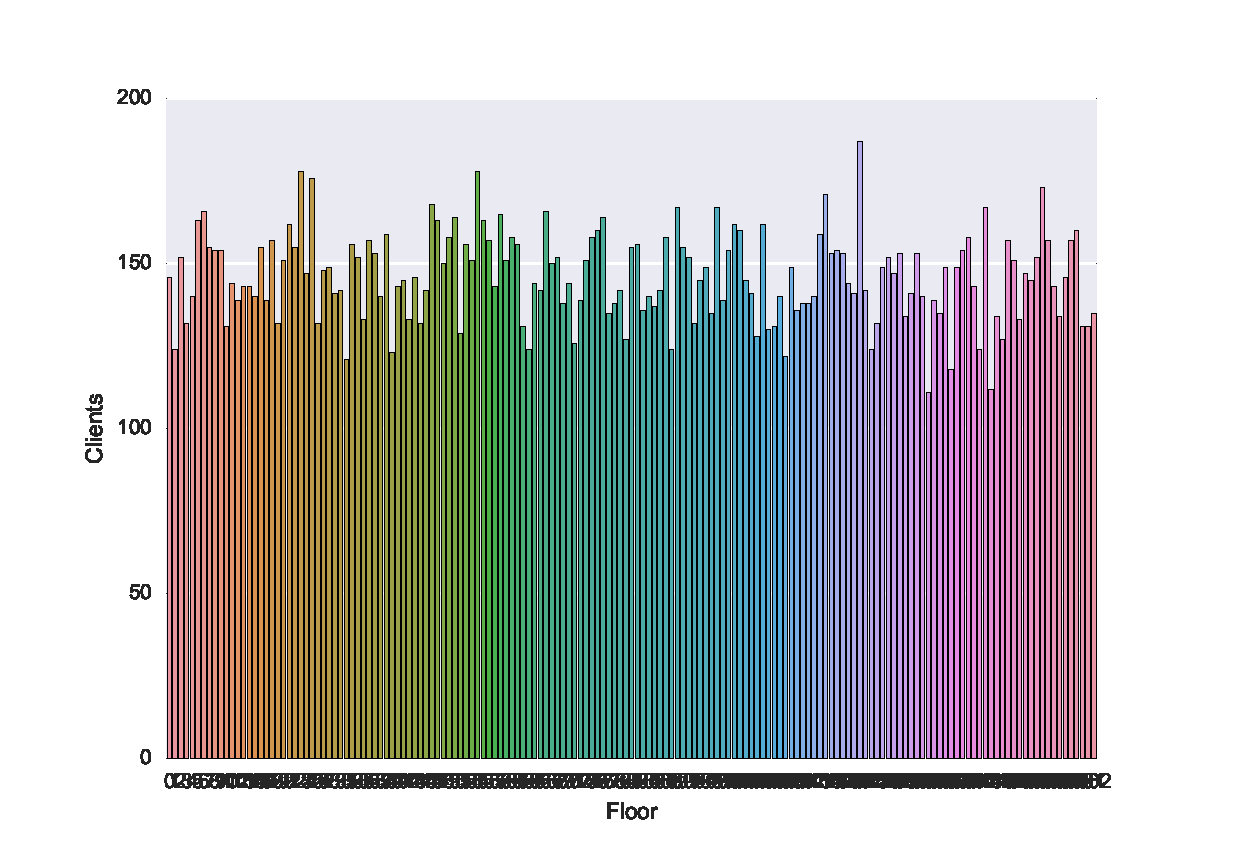
\includegraphics[scale=0.6]{img/results/Low-rise/5_Planning_Random/dropoffsPerFloor.eps}
  \caption{Total de clientes entregues por andar.}
  \label{fig:graphs:dropoffsPerFloor}
\end{figure}

\begin{figure}[htb!]
  \centering
  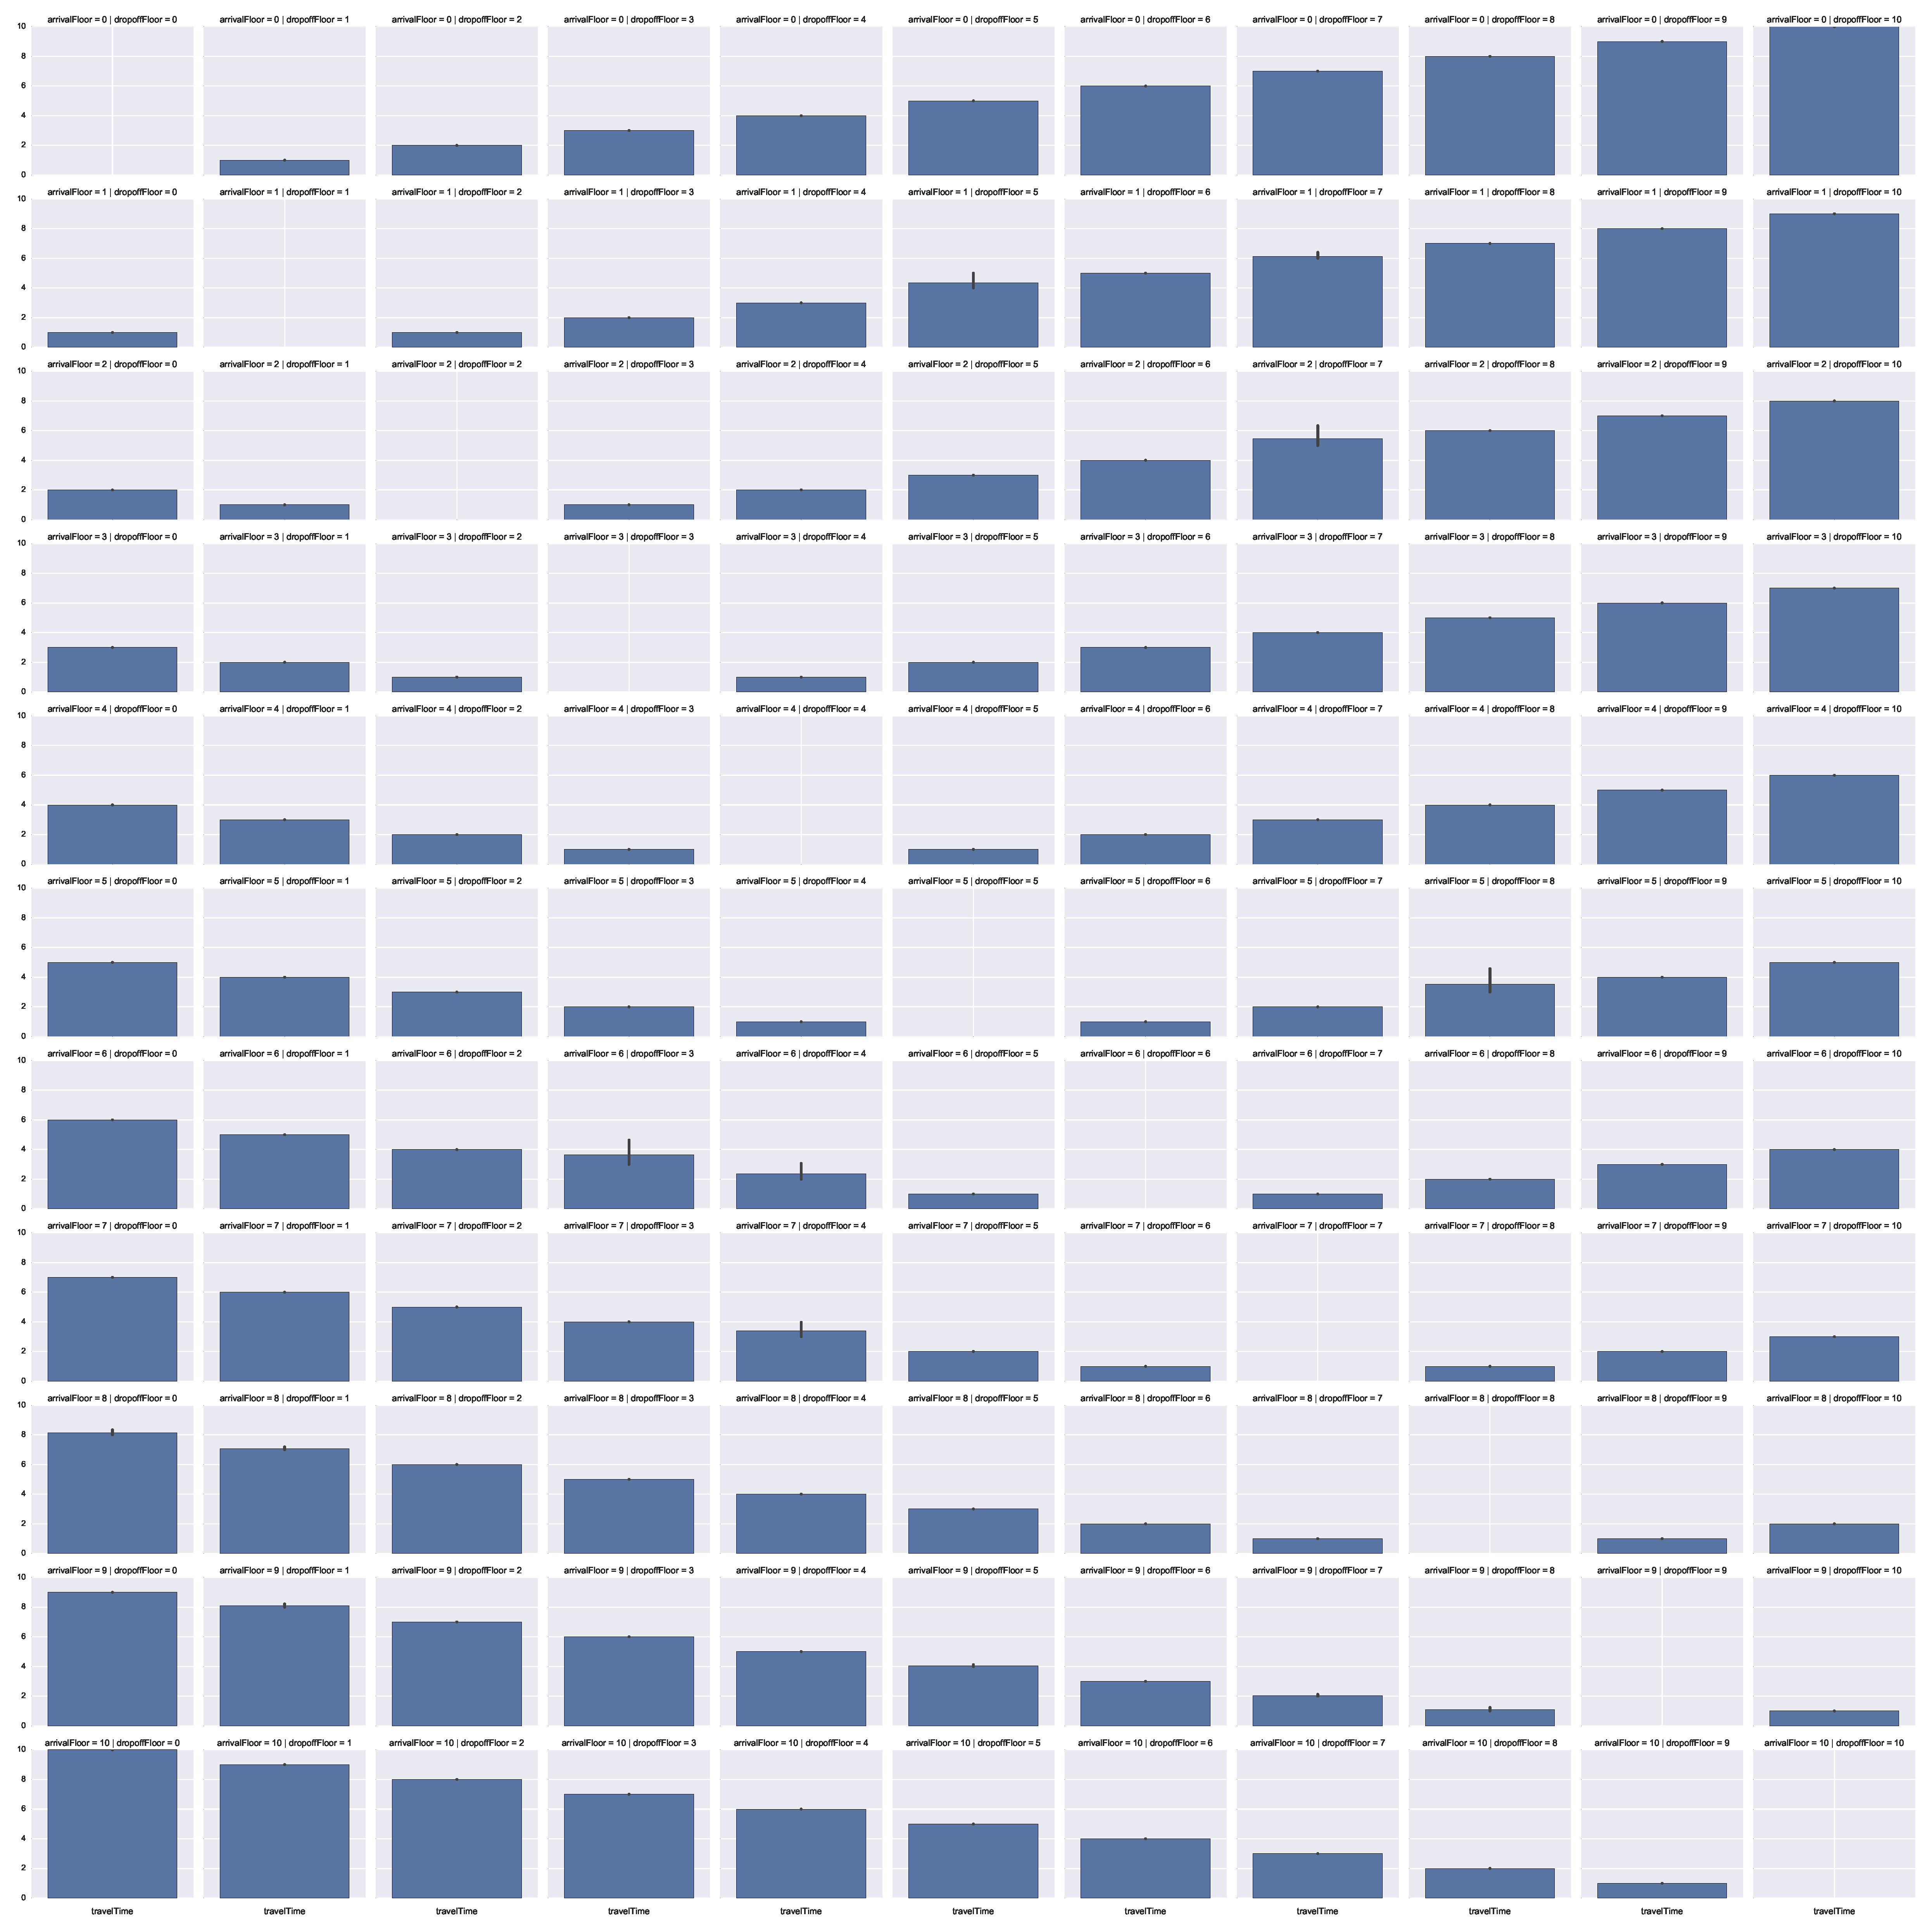
\includegraphics[scale=0.2]{img/results/Low-rise/5_Planning_Random/averageTravelTime.eps}
  \caption{Tempo médio de jornada de andar para andar.}
  \label{fig:graphs:averageTravelTime}
\end{figure}
\chapter{Gráficos de Resultados} \label{app:results}

Além das tabelas e gráficos exibidos no Capítulo~\ref{chap:results}, foram
gerados gráficos para \textit{tempo de espera médio por andar} para cada cenário
e estratégia simulados.

\section{Cenário \textit{Low-rise}.}

\begin{figure}[H]
  \centering
  \includegraphics[scale=0.8]{img/results/Low-rise/1_Simple_Random/averageWaitTime}
  \caption{\textit{Espera média por andar} para \textit{random} e \textit{Low-rise}.}
  \label{fig:result:low-rise:avgwt:random}
\end{figure}

\begin{figure}[H]
  \centering
  \includegraphics[scale=0.8]{img/results/Low-rise/2_Simple_NearestNeighbour/averageWaitTime}
  \caption{\textit{Espera média por andar} para \textit{nearest neighbour} e \textit{Low-rise}.}
  \label{fig:result:low-rise:avgwt:nn}
\end{figure}

\begin{figure}[H]
  \centering
  \includegraphics[scale=0.8]{img/results/Low-rise/3_Simple_BetterNearestNeighbour/averageWaitTime}
  \caption{\textit{Espera média por andar} para \textit{better nearest neighbour} e \textit{Low-rise}.}
  \label{fig:result:low-rise:avgwt:bnn}
\end{figure}

\begin{figure}[H]
  \centering
  \includegraphics[scale=0.8]{img/results/Low-rise/4_Simple_Weighted/averageWaitTime}
  \caption{\textit{Espera média por andar} para \textit{weighted} e \textit{Low-rise}.}
  \label{fig:result:low-rise:avgwt:weighted}
\end{figure}

\begin{figure}[H]
  \centering
  \includegraphics[scale=0.8]{img/results/Low-rise/5_Planning_Random/averageWaitTime}
  \caption{\textit{Espera média por andar} para \textit{planning} e \textit{Low-rise}.}
  \label{fig:result:low-rise:avgwt:planning}
\end{figure}

\section{Cenário \textit{High-rise}.}

\begin{figure}[H]
  \centering
  \includegraphics[scale=0.8]{img/results/High-rise/1_Simple_Random/averageWaitTime}
  \caption{\textit{Espera média por andar} para \textit{random} e \textit{High-rise}.}
  \label{fig:result:high-rise:avgwt:random}
\end{figure}

\begin{figure}[H]
  \centering
  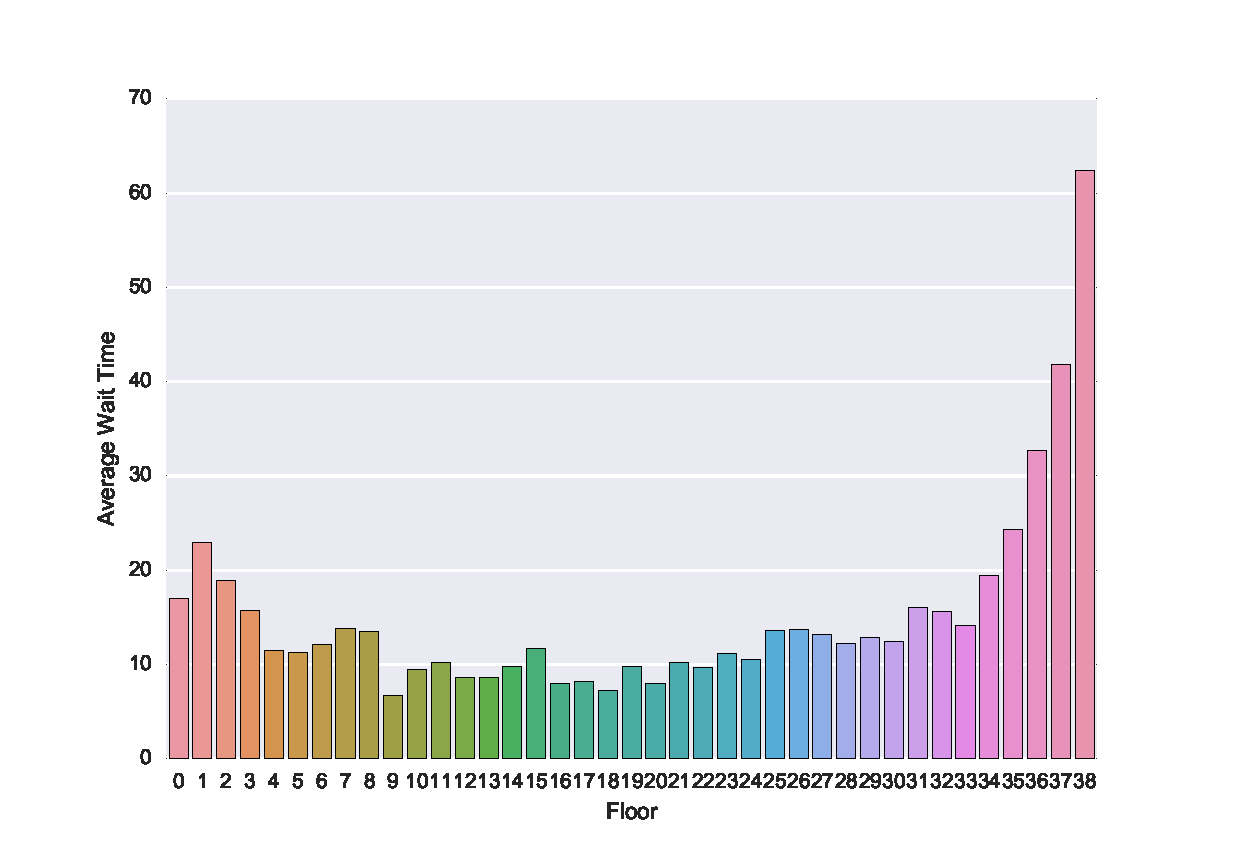
\includegraphics[scale=0.8]{img/results/High-rise/2_Simple_NearestNeighbour/averageWaitTime}
  \caption{\textit{Espera média por andar} para \textit{nearest neighbour} e \textit{High-rise}.}
  \label{fig:result:high-rise:avgwt:nn}
\end{figure}

\begin{figure}[H]
  \centering
  \includegraphics[scale=0.8]{img/results/High-rise/3_Simple_BetterNearestNeighbour/averageWaitTime}
  \caption{\textit{Espera média por andar} para \textit{better nearest neighbour} e \textit{High-rise}.}
  \label{fig:result:high-rise:avgwt:bnn}
\end{figure}

\begin{figure}[H]
  \centering
  \includegraphics[scale=0.8]{img/results/High-rise/4_Simple_Weighted/averageWaitTime}
  \caption{\textit{Espera média por andar} para \textit{weighted} e \textit{High-rise}.}
  \label{fig:result:high-rise:avgwt:weighted}
\end{figure}

\begin{figure}[H]
  \centering
  \includegraphics[scale=0.8]{img/results/High-rise/5_Planning_Random/averageWaitTime}
  \caption{\textit{Espera média por andar} para \textit{planning} e \textit{High-rise}.}
  \label{fig:result:high-rise:avgwt:planning}
\end{figure}

\section{Cenário \textit{Skyscraper}.}

\begin{figure}[H]
  \centering
  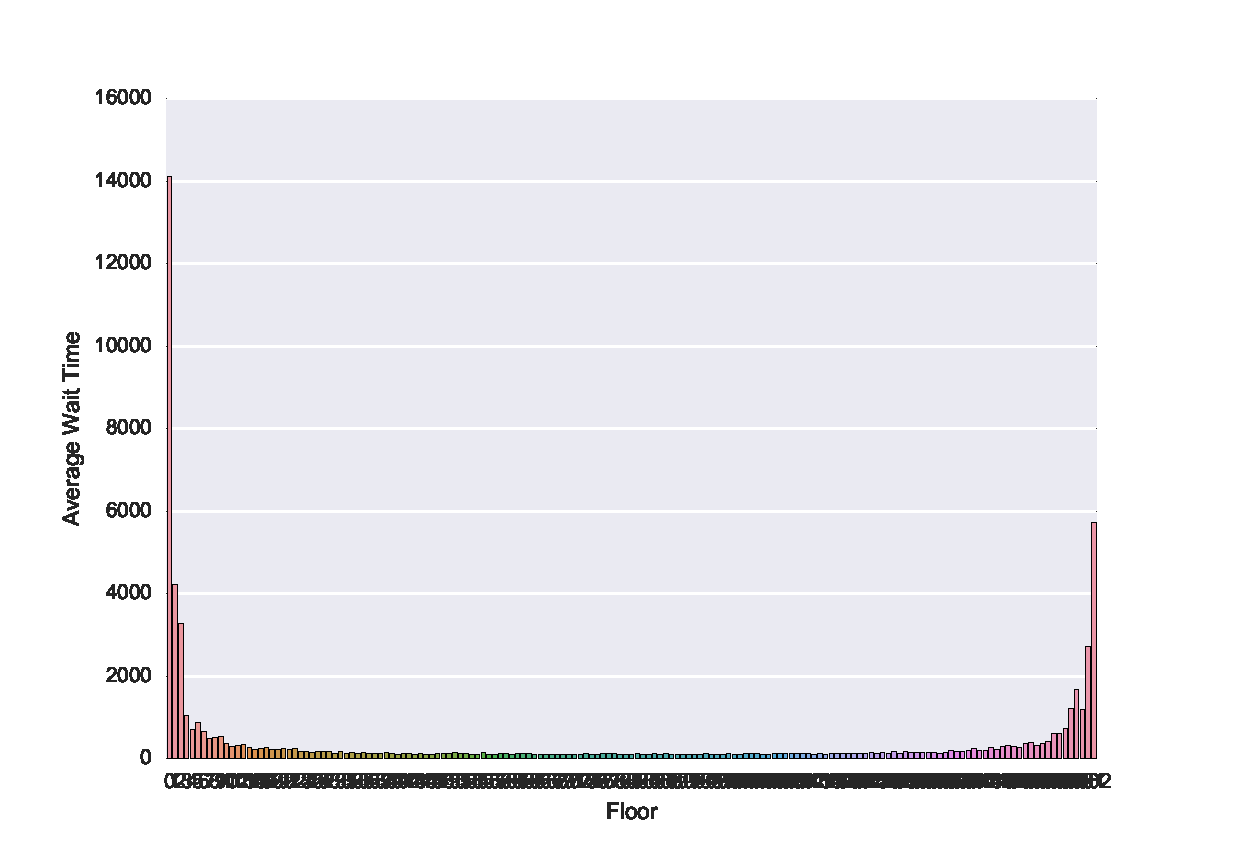
\includegraphics[scale=0.8]{img/results/Skyscraper/1_Simple_Random/averageWaitTime}
  \caption{\textit{Espera média por andar} para \textit{random} e \textit{Skyscraper}.}
  \label{fig:result:skyscraper:avgwt:random}
\end{figure}

\begin{figure}[H]
  \centering
  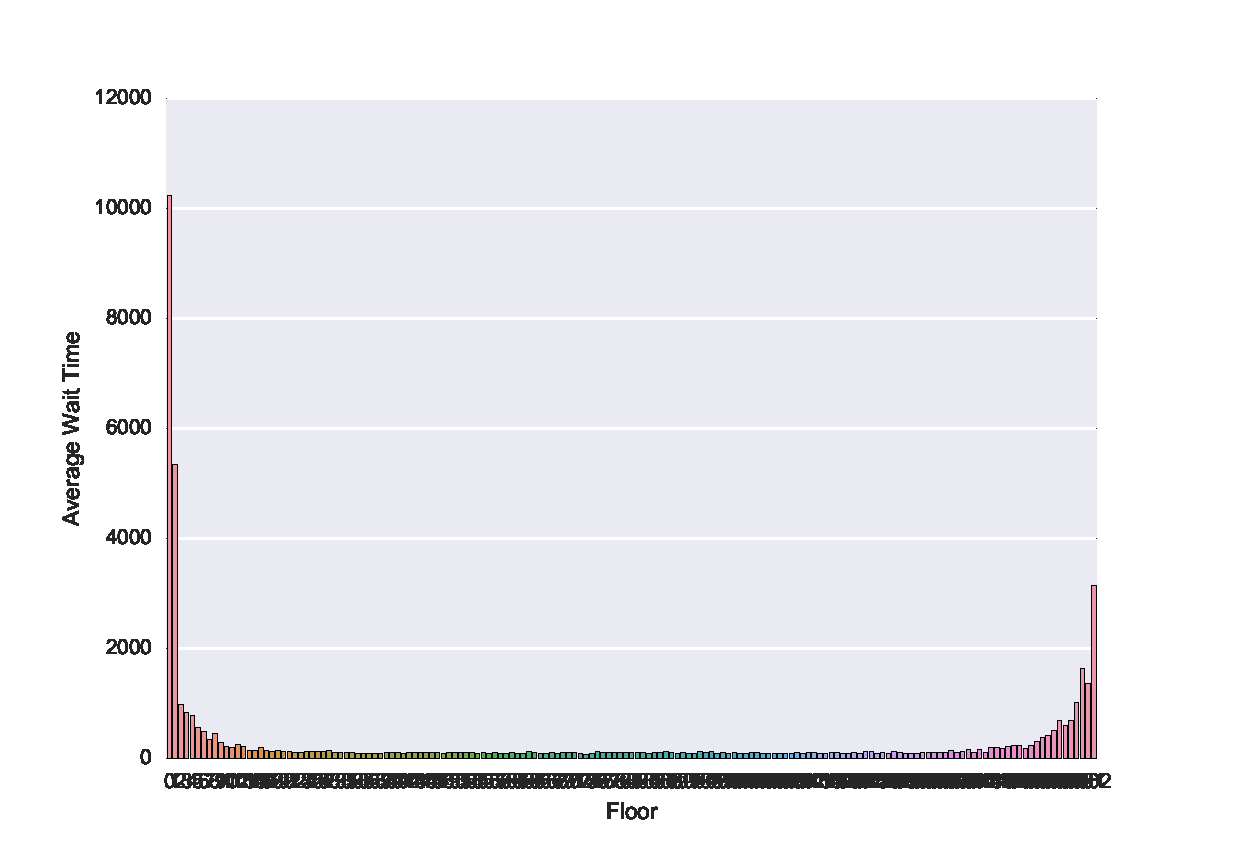
\includegraphics[scale=0.8]{img/results/Skyscraper/2_Simple_NearestNeighbour/averageWaitTime}
  \caption{\textit{Espera média por andar} para \textit{nearest neighbour} e \textit{Skyscraper}.}
  \label{fig:result:skyscraper:avgwt:nn}
\end{figure}

\begin{figure}[H]
  \centering
  \includegraphics[scale=0.8]{img/results/Skyscraper/3_Simple_BetterNearestNeighbour/averageWaitTime}
  \caption{\textit{Espera média por andar} para \textit{better nearest neighbour} e \textit{Skyscraper}.}
  \label{fig:result:skyscraper:avgwt:bnn}
\end{figure}

\begin{figure}[H]
  \centering
  \includegraphics[scale=0.8]{img/results/Skyscraper/4_Simple_Weighted/averageWaitTime}
  \caption{\textit{Espera média por andar} para \textit{weighted} e \textit{Skyscraper}.}
  \label{fig:result:skyscraper:avgwt:weighted}
\end{figure}

\begin{figure}[H]
  \centering
  \includegraphics[scale=0.8]{img/results/Skyscraper/5_Planning_Random/averageWaitTime}
  \caption{\textit{Espera média por andar} para \textit{planning} e \textit{Skyscraper}.}
  \label{fig:result:skyscraper:avgwt:planning}
\end{figure}

\end{document}
